\documentclass{report}

%%%%%%%%%%%%%%%%%%%%%%%%%%%%%%%%%
% PACKAGE IMPORTS
%%%%%%%%%%%%%%%%%%%%%%%%%%%%%%%%%


\usepackage[tmargin=2cm,rmargin=1in,lmargin=1in,margin=0.85in,bmargin=2cm,footskip=.2in]{geometry}
\usepackage{amsmath,amsfonts,amsthm,amssymb,mathtools}
\usepackage[varbb]{newpxmath}
\usepackage{xfrac}
\usepackage[makeroom]{cancel}
\usepackage{mathtools}
\usepackage{bookmark}
\usepackage{enumitem}
\usepackage{hyperref,theoremref}
\hypersetup{
	pdftitle={Assignment},
	colorlinks=true, linkcolor=doc!90,
	bookmarksnumbered=true,
	bookmarksopen=true
}
\usepackage[most,many,breakable]{tcolorbox}
\usepackage{xcolor}
\usepackage{varwidth}
\usepackage{varwidth}
\usepackage{etoolbox}
%\usepackage{authblk}
\usepackage{nameref}
\usepackage{multicol,array}
\usepackage{tikz-cd}
\usepackage[ruled,vlined,linesnumbered]{algorithm2e}
\usepackage{comment} % enables the use of multi-line comments (\ifx \fi) 
\usepackage{import}
\usepackage{xifthen}
\usepackage{pdfpages}
\usepackage{transparent}

% \usepackage{extsizes}

\newcommand\mycommfont[1]{\footnotesize\ttfamily\textcolor{blue}{#1}}
\SetCommentSty{mycommfont}
\newcommand{\incfig}[1]{%
    \def\svgwidth{\columnwidth}
    \import{./figures/}{#1.pdf_tex}
}

\usepackage{tikzsymbols}
\renewcommand\qedsymbol{$\Laughey$}


%\usepackage{import}
%\usepackage{xifthen}
%\usepackage{pdfpages}
%\usepackage{transparent}


%%%%%%%%%%%%%%%%%%%%%%%%%%%%%%
% SELF MADE COLORS
%%%%%%%%%%%%%%%%%%%%%%%%%%%%%%



\definecolor{myg}{RGB}{56, 140, 70}
\definecolor{myb}{RGB}{45, 111, 177}
\definecolor{myr}{RGB}{199, 68, 64}
\definecolor{mytheorembg}{HTML}{F2F2F9}
\definecolor{mytheoremfr}{HTML}{00007B}
\definecolor{mylenmabg}{HTML}{FFFAF8}
\definecolor{mylenmafr}{HTML}{983b0f}
\definecolor{mypropbg}{HTML}{f2fbfc}
\definecolor{mypropfr}{HTML}{191971}
\definecolor{myexamplebg}{HTML}{F2FBF8}
\definecolor{myexamplefr}{HTML}{88D6D1}
\definecolor{myexampleti}{HTML}{2A7F7F}
\definecolor{mydefinitbg}{HTML}{E5E5FF}
\definecolor{mydefinitfr}{HTML}{3F3FA3}
\definecolor{notesgreen}{RGB}{0,162,0}
\definecolor{myp}{RGB}{197, 92, 212}
\definecolor{mygr}{HTML}{2C3338}
\definecolor{myred}{RGB}{127,0,0}
\definecolor{myyellow}{RGB}{169,121,69}
\definecolor{myexercisebg}{HTML}{F2FBF8}
\definecolor{myexercisefg}{HTML}{88D6D1}


%%%%%%%%%%%%%%%%%%%%%%%%%%%%
% TCOLORBOX SETUPS
%%%%%%%%%%%%%%%%%%%%%%%%%%%%

\setlength{\parindent}{1cm}
%================================
% THEOREM BOX
%================================

\tcbuselibrary{theorems,skins,hooks}
\newtcbtheorem[number within=section]{Theorem}{Theorem}
{%
	enhanced,
	breakable,
	colback = mytheorembg,
	frame hidden,
	boxrule = 0sp,
	borderline west = {2pt}{0pt}{mytheoremfr},
	sharp corners,
	detach title,
	before upper = \tcbtitle\par\smallskip,
	coltitle = mytheoremfr,
	fonttitle = \bfseries\sffamily,
	description font = \mdseries,
	separator sign none,
	segmentation style={solid, mytheoremfr},
}
{th}

\tcbuselibrary{theorems,skins,hooks}
\newtcbtheorem[number within=chapter]{theorem}{Theorem}
{%
	enhanced,
	breakable,
	colback = mytheorembg,
	frame hidden,
	boxrule = 0sp,
	borderline west = {2pt}{0pt}{mytheoremfr},
	sharp corners,
	detach title,
	before upper = \tcbtitle\par\smallskip,
	coltitle = mytheoremfr,
	fonttitle = \bfseries\sffamily,
	description font = \mdseries,
	separator sign none,
	segmentation style={solid, mytheoremfr},
}
{th}


\tcbuselibrary{theorems,skins,hooks}
\newtcolorbox{Theoremcon}
{%
	enhanced
	,breakable
	,colback = mytheorembg
	,frame hidden
	,boxrule = 0sp
	,borderline west = {2pt}{0pt}{mytheoremfr}
	,sharp corners
	,description font = \mdseries
	,separator sign none
}

%================================
% Corollery
%================================
\tcbuselibrary{theorems,skins,hooks}
\newtcbtheorem[number within=section]{Corollary}{Corollary}
{%
	enhanced
	,breakable
	,colback = myp!10
	,frame hidden
	,boxrule = 0sp
	,borderline west = {2pt}{0pt}{myp!85!black}
	,sharp corners
	,detach title
	,before upper = \tcbtitle\par\smallskip
	,coltitle = myp!85!black
	,fonttitle = \bfseries\sffamily
	,description font = \mdseries
	,separator sign none
	,segmentation style={solid, myp!85!black}
}
{th}
\tcbuselibrary{theorems,skins,hooks}
\newtcbtheorem[number within=chapter]{corollary}{Corollary}
{%
	enhanced
	,breakable
	,colback = myp!10
	,frame hidden
	,boxrule = 0sp
	,borderline west = {2pt}{0pt}{myp!85!black}
	,sharp corners
	,detach title
	,before upper = \tcbtitle\par\smallskip
	,coltitle = myp!85!black
	,fonttitle = \bfseries\sffamily
	,description font = \mdseries
	,separator sign none
	,segmentation style={solid, myp!85!black}
}
{th}


%================================
% LENMA
%================================

\tcbuselibrary{theorems,skins,hooks}
\newtcbtheorem[number within=section]{Lenma}{Lenma}
{%
	enhanced,
	breakable,
	colback = mylenmabg,
	frame hidden,
	boxrule = 0sp,
	borderline west = {2pt}{0pt}{mylenmafr},
	sharp corners,
	detach title,
	before upper = \tcbtitle\par\smallskip,
	coltitle = mylenmafr,
	fonttitle = \bfseries\sffamily,
	description font = \mdseries,
	separator sign none,
	segmentation style={solid, mylenmafr},
}
{th}

\tcbuselibrary{theorems,skins,hooks}
\newtcbtheorem[number within=chapter]{lenma}{Lenma}
{%
	enhanced,
	breakable,
	colback = mylenmabg,
	frame hidden,
	boxrule = 0sp,
	borderline west = {2pt}{0pt}{mylenmafr},
	sharp corners,
	detach title,
	before upper = \tcbtitle\par\smallskip,
	coltitle = mylenmafr,
	fonttitle = \bfseries\sffamily,
	description font = \mdseries,
	separator sign none,
	segmentation style={solid, mylenmafr},
}
{th}


%================================
% PROPOSITION
%================================

\tcbuselibrary{theorems,skins,hooks}
\newtcbtheorem[number within=section]{Prop}{Proposition}
{%
	enhanced,
	breakable,
	colback = mypropbg,
	frame hidden,
	boxrule = 0sp,
	borderline west = {2pt}{0pt}{mypropfr},
	sharp corners,
	detach title,
	before upper = \tcbtitle\par\smallskip,
	coltitle = mypropfr,
	fonttitle = \bfseries\sffamily,
	description font = \mdseries,
	separator sign none,
	segmentation style={solid, mypropfr},
}
{th}

\tcbuselibrary{theorems,skins,hooks}
\newtcbtheorem[number within=chapter]{prop}{Proposition}
{%
	enhanced,
	breakable,
	colback = mypropbg,
	frame hidden,
	boxrule = 0sp,
	borderline west = {2pt}{0pt}{mypropfr},
	sharp corners,
	detach title,
	before upper = \tcbtitle\par\smallskip,
	coltitle = mypropfr,
	fonttitle = \bfseries\sffamily,
	description font = \mdseries,
	separator sign none,
	segmentation style={solid, mypropfr},
}
{th}


%================================
% CLAIM
%================================

\tcbuselibrary{theorems,skins,hooks}
\newtcbtheorem[number within=section]{claim}{Claim}
{%
	enhanced
	,breakable
	,colback = myg!10
	,frame hidden
	,boxrule = 0sp
	,borderline west = {2pt}{0pt}{myg}
	,sharp corners
	,detach title
	,before upper = \tcbtitle\par\smallskip
	,coltitle = myg!85!black
	,fonttitle = \bfseries\sffamily
	,description font = \mdseries
	,separator sign none
	,segmentation style={solid, myg!85!black}
}
{th}



%================================
% Exercise
%================================

\tcbuselibrary{theorems,skins,hooks}
\newtcbtheorem[number within=section]{Exercise}{Exercise}
{%
	enhanced,
	breakable,
	colback = myexercisebg,
	frame hidden,
	boxrule = 0sp,
	borderline west = {2pt}{0pt}{myexercisefg},
	sharp corners,
	detach title,
	before upper = \tcbtitle\par\smallskip,
	coltitle = myexercisefg,
	fonttitle = \bfseries\sffamily,
	description font = \mdseries,
	separator sign none,
	segmentation style={solid, myexercisefg},
}
{th}

\tcbuselibrary{theorems,skins,hooks}
\newtcbtheorem[number within=chapter]{exercise}{Exercise}
{%
	enhanced,
	breakable,
	colback = myexercisebg,
	frame hidden,
	boxrule = 0sp,
	borderline west = {2pt}{0pt}{myexercisefg},
	sharp corners,
	detach title,
	before upper = \tcbtitle\par\smallskip,
	coltitle = myexercisefg,
	fonttitle = \bfseries\sffamily,
	description font = \mdseries,
	separator sign none,
	segmentation style={solid, myexercisefg},
}
{th}

%================================
% EXAMPLE BOX
%================================

\newtcbtheorem[number within=section]{Example}{Example}
{%
	colback = myexamplebg
	,breakable
	,colframe = myexamplefr
	,coltitle = myexampleti
	,boxrule = 1pt
	,sharp corners
	,detach title
	,before upper=\tcbtitle\par\smallskip
	,fonttitle = \bfseries
	,description font = \mdseries
	,separator sign none
	,description delimiters parenthesis
}
{ex}

\newtcbtheorem[number within=chapter]{example}{Example}
{%
	colback = myexamplebg
	,breakable
	,colframe = myexamplefr
	,coltitle = myexampleti
	,boxrule = 1pt
	,sharp corners
	,detach title
	,before upper=\tcbtitle\par\smallskip
	,fonttitle = \bfseries
	,description font = \mdseries
	,separator sign none
	,description delimiters parenthesis
}
{ex}

%================================
% DEFINITION BOX
%================================

\newtcbtheorem[number within=section]{Definition}{Definition}{enhanced,
	before skip=2mm,after skip=2mm, colback=red!5,colframe=red!80!black,boxrule=0.5mm,
	attach boxed title to top left={xshift=1cm,yshift*=1mm-\tcboxedtitleheight}, varwidth boxed title*=-3cm,
	boxed title style={frame code={
					\path[fill=tcbcolback]
					([yshift=-1mm,xshift=-1mm]frame.north west)
					arc[start angle=0,end angle=180,radius=1mm]
					([yshift=-1mm,xshift=1mm]frame.north east)
					arc[start angle=180,end angle=0,radius=1mm];
					\path[left color=tcbcolback!60!black,right color=tcbcolback!60!black,
						middle color=tcbcolback!80!black]
					([xshift=-2mm]frame.north west) -- ([xshift=2mm]frame.north east)
					[rounded corners=1mm]-- ([xshift=1mm,yshift=-1mm]frame.north east)
					-- (frame.south east) -- (frame.south west)
					-- ([xshift=-1mm,yshift=-1mm]frame.north west)
					[sharp corners]-- cycle;
				},interior engine=empty,
		},
	fonttitle=\bfseries,
	title={#2},#1}{def}
\newtcbtheorem[number within=chapter]{definition}{Definition}{enhanced,
	before skip=2mm,after skip=2mm, colback=red!5,colframe=red!80!black,boxrule=0.5mm,
	attach boxed title to top left={xshift=1cm,yshift*=1mm-\tcboxedtitleheight}, varwidth boxed title*=-3cm,
	boxed title style={frame code={
					\path[fill=tcbcolback]
					([yshift=-1mm,xshift=-1mm]frame.north west)
					arc[start angle=0,end angle=180,radius=1mm]
					([yshift=-1mm,xshift=1mm]frame.north east)
					arc[start angle=180,end angle=0,radius=1mm];
					\path[left color=tcbcolback!60!black,right color=tcbcolback!60!black,
						middle color=tcbcolback!80!black]
					([xshift=-2mm]frame.north west) -- ([xshift=2mm]frame.north east)
					[rounded corners=1mm]-- ([xshift=1mm,yshift=-1mm]frame.north east)
					-- (frame.south east) -- (frame.south west)
					-- ([xshift=-1mm,yshift=-1mm]frame.north west)
					[sharp corners]-- cycle;
				},interior engine=empty,
		},
	fonttitle=\bfseries,
	title={#2},#1}{def}



%================================
% Solution BOX
%================================

\makeatletter
\newtcbtheorem{question}{Question}{enhanced,
	breakable,
	colback=white,
	colframe=myb!80!black,
	attach boxed title to top left={yshift*=-\tcboxedtitleheight},
	fonttitle=\bfseries,
	title={#2},
	boxed title size=title,
	boxed title style={%
			sharp corners,
			rounded corners=northwest,
			colback=tcbcolframe,
			boxrule=0pt,
		},
	underlay boxed title={%
			\path[fill=tcbcolframe] (title.south west)--(title.south east)
			to[out=0, in=180] ([xshift=5mm]title.east)--
			(title.center-|frame.east)
			[rounded corners=\kvtcb@arc] |-
			(frame.north) -| cycle;
		},
	#1
}{def}
\makeatother

%================================
% SOLUTION BOX
%================================

\makeatletter
\newtcolorbox{solution}{enhanced,
	breakable,
	colback=white,
	colframe=myg!80!black,
	attach boxed title to top left={yshift*=-\tcboxedtitleheight},
	title=Solution,
	boxed title size=title,
	boxed title style={%
			sharp corners,
			rounded corners=northwest,
			colback=tcbcolframe,
			boxrule=0pt,
		},
	underlay boxed title={%
			\path[fill=tcbcolframe] (title.south west)--(title.south east)
			to[out=0, in=180] ([xshift=5mm]title.east)--
			(title.center-|frame.east)
			[rounded corners=\kvtcb@arc] |-
			(frame.north) -| cycle;
		},
}
\makeatother

%================================
% Question BOX
%================================

\makeatletter
\newtcbtheorem{qstion}{Question}{enhanced,
	breakable,
	colback=white,
	colframe=mygr,
	attach boxed title to top left={yshift*=-\tcboxedtitleheight},
	fonttitle=\bfseries,
	title={#2},
	boxed title size=title,
	boxed title style={%
			sharp corners,
			rounded corners=northwest,
			colback=tcbcolframe,
			boxrule=0pt,
		},
	underlay boxed title={%
			\path[fill=tcbcolframe] (title.south west)--(title.south east)
			to[out=0, in=180] ([xshift=5mm]title.east)--
			(title.center-|frame.east)
			[rounded corners=\kvtcb@arc] |-
			(frame.north) -| cycle;
		},
	#1
}{def}
\makeatother

\newtcbtheorem[number within=chapter]{wconc}{Wrong Concept}{
	breakable,
	enhanced,
	colback=white,
	colframe=myr,
	arc=0pt,
	outer arc=0pt,
	fonttitle=\bfseries\sffamily\large,
	colbacktitle=myr,
	attach boxed title to top left={},
	boxed title style={
			enhanced,
			skin=enhancedfirst jigsaw,
			arc=3pt,
			bottom=0pt,
			interior style={fill=myr}
		},
	#1
}{def}



%================================
% NOTE BOX
%================================

\usetikzlibrary{arrows,calc,shadows.blur}
\tcbuselibrary{skins}
\newtcolorbox{note}[1][]{%
	enhanced jigsaw,
	colback=gray!20!white,%
	colframe=gray!80!black,
	size=small,
	boxrule=1pt,
	title=\textbf{Note:},
	halign title=flush center,
	coltitle=black,
	breakable,
	drop shadow=black!50!white,
	attach boxed title to top left={xshift=1cm,yshift=-\tcboxedtitleheight/2,yshifttext=-\tcboxedtitleheight/2},
	minipage boxed title=1.5cm,
	boxed title style={%
			colback=white,
			size=fbox,
			boxrule=1pt,
			boxsep=2pt,
			underlay={%
					\coordinate (dotA) at ($(interior.west) + (-0.5pt,0)$);
					\coordinate (dotB) at ($(interior.east) + (0.5pt,0)$);
					\begin{scope}
						\clip (interior.north west) rectangle ([xshift=3ex]interior.east);
						\filldraw [white, blur shadow={shadow opacity=60, shadow yshift=-.75ex}, rounded corners=2pt] (interior.north west) rectangle (interior.south east);
					\end{scope}
					\begin{scope}[gray!80!black]
						\fill (dotA) circle (2pt);
						\fill (dotB) circle (2pt);
					\end{scope}
				},
		},
	#1,
}

%%%%%%%%%%%%%%%%%%%%%%%%%%%%%%
% SELF MADE COMMANDS
%%%%%%%%%%%%%%%%%%%%%%%%%%%%%%


\newcommand{\thm}[2]{\begin{Theorem}{#1}{}#2\end{Theorem}}
\newcommand{\cor}[2]{\begin{Corollary}{#1}{}#2\end{Corollary}}
\newcommand{\mlenma}[2]{\begin{Lenma}{#1}{}#2\end{Lenma}}
\newcommand{\mprop}[2]{\begin{Prop}{#1}{}#2\end{Prop}}
\newcommand{\clm}[3]{\begin{claim}{#1}{#2}#3\end{claim}}
\newcommand{\wc}[2]{\begin{wconc}{#1}{}\setlength{\parindent}{1cm}#2\end{wconc}}
\newcommand{\thmcon}[1]{\begin{Theoremcon}{#1}\end{Theoremcon}}
\newcommand{\ex}[2]{\begin{Example}{#1}{}#2\end{Example}}
\newcommand{\dfn}[2]{\begin{Definition}[colbacktitle=red!75!black]{#1}{}#2\end{Definition}}
\newcommand{\dfnc}[2]{\begin{definition}[colbacktitle=red!75!black]{#1}{}#2\end{definition}}
\newcommand{\qs}[2]{\begin{question*}{#1}{}#2\end{question*}}
\newcommand{\mpf}[2]{\begin{myproof}[#1]#2\end{myproof}}
\newcommand{\nt}[1]{\begin{note}#1\end{note}}

\newcommand*\circled[1]{\tikz[baseline=(char.base)]{
		\node[shape=circle,draw,inner sep=1pt] (char) {#1};}}
\newcommand\getcurrentref[1]{%
	\ifnumequal{\value{#1}}{0}
	{??}
	{\the\value{#1}}%
}
\newcommand{\getCurrentSectionNumber}{\getcurrentref{section}}
\newenvironment{myproof}[1][\proofname]{%
	\proof[\bfseries #1: ]%
}{\endproof}

\newcommand{\mclm}[2]{\begin{myclaim}[#1]#2\end{myclaim}}
\newenvironment{myclaim}[1][\claimname]{\proof[\bfseries #1: ]}{}

\newcounter{mylabelcounter}

\makeatletter
\newcommand{\setword}[2]{%
	\phantomsection
	#1\def\@currentlabel{\unexpanded{#1}}\label{#2}%
}
\makeatother




\tikzset{
	symbol/.style={
			draw=none,
			every to/.append style={
					edge node={node [sloped, allow upside down, auto=false]{$#1$}}}
		}
}


% deliminators
\DeclarePairedDelimiter{\abs}{\lvert}{\rvert}
\DeclarePairedDelimiter{\norm}{\lVert}{\rVert}

\DeclarePairedDelimiter{\ceil}{\lceil}{\rceil}
\DeclarePairedDelimiter{\floor}{\lfloor}{\rfloor}
\DeclarePairedDelimiter{\round}{\lfloor}{\rceil}

\newsavebox\diffdbox
\newcommand{\slantedromand}{{\mathpalette\makesl{d}}}
\newcommand{\makesl}[2]{%
\begingroup
\sbox{\diffdbox}{$\mathsurround=0pt#1\mathrm{#2}$}%
\pdfsave
\pdfsetmatrix{1 0 0.2 1}%
\rlap{\usebox{\diffdbox}}%
\pdfrestore
\hskip\wd\diffdbox
\endgroup
}
\newcommand{\dd}[1][]{\ensuremath{\mathop{}\!\ifstrempty{#1}{%
\slantedromand\@ifnextchar^{\hspace{0.2ex}}{\hspace{0.1ex}}}%
{\slantedromand\hspace{0.2ex}^{#1}}}}
\ProvideDocumentCommand\dv{o m g}{%
  \ensuremath{%
    \IfValueTF{#3}{%
      \IfNoValueTF{#1}{%
        \frac{\dd #2}{\dd #3}%
      }{%
        \frac{\dd^{#1} #2}{\dd #3^{#1}}%
      }%
    }{%
      \IfNoValueTF{#1}{%
        \frac{\dd}{\dd #2}%
      }{%
        \frac{\dd^{#1}}{\dd #2^{#1}}%
      }%
    }%
  }%
}
\providecommand*{\pdv}[3][]{\frac{\partial^{#1}#2}{\partial#3^{#1}}}
%  - others
\DeclareMathOperator{\Lap}{\mathcal{L}}
\DeclareMathOperator{\Var}{Var} % varience
\DeclareMathOperator{\Cov}{Cov} % covarience
\DeclareMathOperator{\E}{E} % expected

% Since the amsthm package isn't loaded

% I prefer the slanted \leq
\let\oldleq\leq % save them in case they're every wanted
\let\oldgeq\geq
\renewcommand{\leq}{\leqslant}
\renewcommand{\geq}{\geqslant}

% % redefine matrix env to allow for alignment, use r as default
% \renewcommand*\env@matrix[1][r]{\hskip -\arraycolsep
%     \let\@ifnextchar\new@ifnextchar
%     \array{*\c@MaxMatrixCols #1}}


%\usepackage{framed}
%\usepackage{titletoc}
%\usepackage{etoolbox}
%\usepackage{lmodern}


%\patchcmd{\tableofcontents}{\contentsname}{\sffamily\contentsname}{}{}

%\renewenvironment{leftbar}
%{\def\FrameCommand{\hspace{6em}%
%		{\color{myyellow}\vrule width 2pt depth 6pt}\hspace{1em}}%
%	\MakeFramed{\parshape 1 0cm \dimexpr\textwidth-6em\relax\FrameRestore}\vskip2pt%
%}
%{\endMakeFramed}

%\titlecontents{chapter}
%[0em]{\vspace*{2\baselineskip}}
%{\parbox{4.5em}{%
%		\hfill\Huge\sffamily\bfseries\color{myred}\thecontentspage}%
%	\vspace*{-2.3\baselineskip}\leftbar\textsc{\small\chaptername~\thecontentslabel}\\\sffamily}
%{}{\endleftbar}
%\titlecontents{section}
%[8.4em]
%{\sffamily\contentslabel{3em}}{}{}
%{\hspace{0.5em}\nobreak\itshape\color{myred}\contentspage}
%\titlecontents{subsection}
%[8.4em]
%{\sffamily\contentslabel{3em}}{}{}  
%{\hspace{0.5em}\nobreak\itshape\color{myred}\contentspage}



%%%%%%%%%%%%%%%%%%%%%%%%%%%%%%%%%%%%%%%%%%%
% TABLE OF CONTENTS
%%%%%%%%%%%%%%%%%%%%%%%%%%%%%%%%%%%%%%%%%%%

\usepackage{tikz}
\definecolor{doc}{RGB}{0,60,110}
\usepackage{titletoc}
\contentsmargin{0cm}
\titlecontents{chapter}[3.7pc]
{\addvspace{30pt}%
	\begin{tikzpicture}[remember picture, overlay]%
		\draw[fill=doc!60,draw=doc!60] (-7,-.1) rectangle (-0.9,.5);%
		\pgftext[left,x=-3.5cm,y=0.2cm]{\color{white}\Large\sc\bfseries Chapter\ \thecontentslabel};%
	\end{tikzpicture}\color{doc!60}\large\sc\bfseries}%
{}
{}
{\;\titlerule\;\large\sc\bfseries Page \thecontentspage
	\begin{tikzpicture}[remember picture, overlay]
		\draw[fill=doc!60,draw=doc!60] (2pt,0) rectangle (4,0.1pt);
	\end{tikzpicture}}%
\titlecontents{section}[3.7pc]
{\addvspace{2pt}}
{\contentslabel[\thecontentslabel]{2pc}}
{}
{\hfill\small \thecontentspage}
[]
\titlecontents*{subsection}[3.7pc]
{\addvspace{-1pt}\small}
{}
{}
{\ --- \small\thecontentspage}
[ \textbullet\ ][]

\makeatletter
\renewcommand{\tableofcontents}{%
	\chapter*{%
	  \vspace*{-20\p@}%
	  \begin{tikzpicture}[remember picture, overlay]%
		  \pgftext[right,x=15cm,y=0.2cm]{\color{doc!60}\Huge\sc\bfseries \contentsname};%
		  \draw[fill=doc!60,draw=doc!60] (13,-.75) rectangle (20,1);%
		  \clip (13,-.75) rectangle (20,1);
		  \pgftext[right,x=15cm,y=0.2cm]{\color{white}\Huge\sc\bfseries \contentsname};%
	  \end{tikzpicture}}%
	\@starttoc{toc}}
\makeatother
\newcommand{\id}{\mathrm{id}}
\newcommand{\taking}[1]{\xrightarrow{#1}}
\newcommand{\inv}{^{-1}}

%From M170 "Introduction to Graph Theory" at SJSU
\DeclareMathOperator{\diam}{diam}
\DeclareMathOperator{\ord}{ord}
\newcommand{\defeq}{\overset{\mathrm{def}}{=}}

%From the USAMO .tex files
\newcommand{\ts}{\textsuperscript}
\newcommand{\dg}{^\circ}
\newcommand{\ii}{\item}

% % From Math 55 and Math 145 at Harvard
% \newenvironment{subproof}[1][Proof]{%
% \begin{proof}[#1] \renewcommand{\qedsymbol}{$\blacksquare$}}%
% {\end{proof}}

\newcommand{\liff}{\leftrightarrow}
\newcommand{\lthen}{\rightarrow}
\newcommand{\opname}{\operatorname}
\newcommand{\surjto}{\twoheadrightarrow}
\newcommand{\injto}{\hookrightarrow}
\newcommand{\On}{\mathrm{On}} % ordinals
\DeclareMathOperator{\img}{im} % Image
\DeclareMathOperator{\Img}{Im} % Image
\DeclareMathOperator{\coker}{coker} % Cokernel
\DeclareMathOperator{\Coker}{Coker} % Cokernel
\DeclareMathOperator{\Ker}{Ker} % Kernel
\DeclareMathOperator{\rank}{rank}
\DeclareMathOperator{\Spec}{Spec} % spectrum
\DeclareMathOperator{\Tr}{Tr} % trace
\DeclareMathOperator{\pr}{pr} % projection
\DeclareMathOperator{\ext}{ext} % extension
\DeclareMathOperator{\pred}{pred} % predecessor
\DeclareMathOperator{\dom}{dom} % domain
\DeclareMathOperator{\ran}{ran} % range
\DeclareMathOperator{\Hom}{Hom} % homomorphism
\DeclareMathOperator{\Mor}{Mor} % morphisms
\DeclareMathOperator{\End}{End} % endomorphism

\newcommand{\eps}{\epsilon}
\newcommand{\veps}{\varepsilon}
\newcommand{\ol}{\overline}
\newcommand{\ul}{\underline}
\newcommand{\wt}{\widetilde}
\newcommand{\wh}{\widehat}
\newcommand{\vocab}[1]{\textbf{\color{blue} #1}}
\providecommand{\half}{\frac{1}{2}}
\newcommand{\dang}{\measuredangle} %% Directed angle
\newcommand{\ray}[1]{\overrightarrow{#1}}
\newcommand{\seg}[1]{\overline{#1}}
\newcommand{\arc}[1]{\wideparen{#1}}
\DeclareMathOperator{\cis}{cis}
\DeclareMathOperator*{\lcm}{lcm}
\DeclareMathOperator*{\argmin}{arg min}
\DeclareMathOperator*{\argmax}{arg max}
\newcommand{\cycsum}{\sum_{\mathrm{cyc}}}
\newcommand{\symsum}{\sum_{\mathrm{sym}}}
\newcommand{\cycprod}{\prod_{\mathrm{cyc}}}
\newcommand{\symprod}{\prod_{\mathrm{sym}}}
\newcommand{\Qed}{\begin{flushright}\qed\end{flushright}}
\newcommand{\parinn}{\setlength{\parindent}{1cm}}
\newcommand{\parinf}{\setlength{\parindent}{0cm}}
% \newcommand{\norm}{\|\cdot\|}
\newcommand{\inorm}{\norm_{\infty}}
\newcommand{\opensets}{\{V_{\alpha}\}_{\alpha\in I}}
\newcommand{\oset}{V_{\alpha}}
\newcommand{\opset}[1]{V_{\alpha_{#1}}}
\newcommand{\lub}{\text{lub}}
\newcommand{\del}[2]{\frac{\partial #1}{\partial #2}}
\newcommand{\Del}[3]{\frac{\partial^{#1} #2}{\partial^{#1} #3}}
\newcommand{\deld}[2]{\dfrac{\partial #1}{\partial #2}}
\newcommand{\Deld}[3]{\dfrac{\partial^{#1} #2}{\partial^{#1} #3}}
\newcommand{\lm}{\lambda}
\newcommand{\uin}{\mathbin{\rotatebox[origin=c]{90}{$\in$}}}
\newcommand{\usubset}{\mathbin{\rotatebox[origin=c]{90}{$\subset$}}}
\newcommand{\lt}{\left}
\newcommand{\rt}{\right}
\newcommand{\bs}[1]{\boldsymbol{#1}}
\newcommand{\exs}{\exists}
\newcommand{\st}{\strut}
\newcommand{\dps}[1]{\displaystyle{#1}}

\newcommand{\sol}{\setlength{\parindent}{0cm}\textbf{\textit{Solution:}}\setlength{\parindent}{1cm} }
\newcommand{\solve}[1]{\setlength{\parindent}{0cm}\textbf{\textit{Solution: }}\setlength{\parindent}{1cm}#1 \Qed}
% Things Lie
\newcommand{\kb}{\mathfrak b}
\newcommand{\kg}{\mathfrak g}
\newcommand{\kh}{\mathfrak h}
\newcommand{\kn}{\mathfrak n}
\newcommand{\ku}{\mathfrak u}
\newcommand{\kz}{\mathfrak z}
\DeclareMathOperator{\Ext}{Ext} % Ext functor
\DeclareMathOperator{\Tor}{Tor} % Tor functor
\newcommand{\gl}{\opname{\mathfrak{gl}}} % frak gl group
\renewcommand{\sl}{\opname{\mathfrak{sl}}} % frak sl group chktex 6

% More script letters etc.
\newcommand{\SA}{\mathcal A}
\newcommand{\SB}{\mathcal B}
\newcommand{\SC}{\mathcal C}
\newcommand{\SF}{\mathcal F}
\newcommand{\SG}{\mathcal G}
\newcommand{\SH}{\mathcal H}
\newcommand{\OO}{\mathcal O}

\newcommand{\SCA}{\mathscr A}
\newcommand{\SCB}{\mathscr B}
\newcommand{\SCC}{\mathscr C}
\newcommand{\SCD}{\mathscr D}
\newcommand{\SCE}{\mathscr E}
\newcommand{\SCF}{\mathscr F}
\newcommand{\SCG}{\mathscr G}
\newcommand{\SCH}{\mathscr H}

% Mathfrak primes
\newcommand{\km}{\mathfrak m}
\newcommand{\kp}{\mathfrak p}
\newcommand{\kq}{\mathfrak q}

% number sets
\newcommand{\RR}[1][]{\ensuremath{\ifstrempty{#1}{\mathbb{R}}{\mathbb{R}^{#1}}}}
\newcommand{\NN}[1][]{\ensuremath{\ifstrempty{#1}{\mathbb{N}}{\mathbb{N}^{#1}}}}
\newcommand{\ZZ}[1][]{\ensuremath{\ifstrempty{#1}{\mathbb{Z}}{\mathbb{Z}^{#1}}}}
\newcommand{\QQ}[1][]{\ensuremath{\ifstrempty{#1}{\mathbb{Q}}{\mathbb{Q}^{#1}}}}
\newcommand{\CC}[1][]{\ensuremath{\ifstrempty{#1}{\mathbb{C}}{\mathbb{C}^{#1}}}}
\newcommand{\PP}[1][]{\ensuremath{\ifstrempty{#1}{\mathbb{P}}{\mathbb{P}^{#1}}}}
\newcommand{\HH}[1][]{\ensuremath{\ifstrempty{#1}{\mathbb{H}}{\mathbb{H}^{#1}}}}
\newcommand{\FF}[1][]{\ensuremath{\ifstrempty{#1}{\mathbb{F}}{\mathbb{F}^{#1}}}}

% number sets without arguments
\newcommand{\R}{\ensuremath{\mathbb{R}}}
\newcommand{\N}{\ensuremath{\mathbb{N}}}
\newcommand{\Z}{\ensuremath{\mathbb{Z}}}
\newcommand{\Q}{\ensuremath{\mathbb{Q}}}
\newcommand{\C}{\ensuremath{\mathbb{C}}}
\newcommand{\F}{\ensuremath{\mathbb{F}}}

% expected value
\newcommand{\EE}{\ensuremath{\mathbb{E}}}
\newcommand{\charin}{\text{ char }}
\DeclareMathOperator{\sign}{sign}
\DeclareMathOperator{\Aut}{Aut}
\DeclareMathOperator{\Inn}{Inn}
\DeclareMathOperator{\Syl}{Syl}
\DeclareMathOperator{\Gal}{Gal}
\DeclareMathOperator{\GL}{GL} % General linear group
\DeclareMathOperator{\SL}{SL} % Special linear group

%---------------------------------------
% BlackBoard Math Fonts :-
%---------------------------------------

%Captital Letters
\newcommand{\bbA}{\mathbb{A}}	\newcommand{\bbB}{\mathbb{B}}
\newcommand{\bbC}{\mathbb{C}}	\newcommand{\bbD}{\mathbb{D}}
\newcommand{\bbE}{\mathbb{E}}	\newcommand{\bbF}{\mathbb{F}}
\newcommand{\bbG}{\mathbb{G}}	\newcommand{\bbH}{\mathbb{H}}
\newcommand{\bbI}{\mathbb{I}}	\newcommand{\bbJ}{\mathbb{J}}
\newcommand{\bbK}{\mathbb{K}}	\newcommand{\bbL}{\mathbb{L}}
\newcommand{\bbM}{\mathbb{M}}	\newcommand{\bbN}{\mathbb{N}}
\newcommand{\bbO}{\mathbb{O}}	\newcommand{\bbP}{\mathbb{P}}
\newcommand{\bbQ}{\mathbb{Q}}	\newcommand{\bbR}{\mathbb{R}}
\newcommand{\bbS}{\mathbb{S}}	\newcommand{\bbT}{\mathbb{T}}
\newcommand{\bbU}{\mathbb{U}}	\newcommand{\bbV}{\mathbb{V}}
\newcommand{\bbW}{\mathbb{W}}	\newcommand{\bbX}{\mathbb{X}}
\newcommand{\bbY}{\mathbb{Y}}	\newcommand{\bbZ}{\mathbb{Z}}

%---------------------------------------
% MathCal Fonts :-
%---------------------------------------

%Captital Letters
\newcommand{\mcA}{\mathcal{A}}	\newcommand{\mcB}{\mathcal{B}}
\newcommand{\mcC}{\mathcal{C}}	\newcommand{\mcD}{\mathcal{D}}
\newcommand{\mcE}{\mathcal{E}}	\newcommand{\mcF}{\mathcal{F}}
\newcommand{\mcG}{\mathcal{G}}	\newcommand{\mcH}{\mathcal{H}}
\newcommand{\mcI}{\mathcal{I}}	\newcommand{\mcJ}{\mathcal{J}}
\newcommand{\mcK}{\mathcal{K}}	\newcommand{\mcL}{\mathcal{L}}
\newcommand{\mcM}{\mathcal{M}}	\newcommand{\mcN}{\mathcal{N}}
\newcommand{\mcO}{\mathcal{O}}	\newcommand{\mcP}{\mathcal{P}}
\newcommand{\mcQ}{\mathcal{Q}}	\newcommand{\mcR}{\mathcal{R}}
\newcommand{\mcS}{\mathcal{S}}	\newcommand{\mcT}{\mathcal{T}}
\newcommand{\mcU}{\mathcal{U}}	\newcommand{\mcV}{\mathcal{V}}
\newcommand{\mcW}{\mathcal{W}}	\newcommand{\mcX}{\mathcal{X}}
\newcommand{\mcY}{\mathcal{Y}}	\newcommand{\mcZ}{\mathcal{Z}}


%---------------------------------------
% Bold Math Fonts :-
%---------------------------------------

%Captital Letters
\newcommand{\bmA}{\boldsymbol{A}}	\newcommand{\bmB}{\boldsymbol{B}}
\newcommand{\bmC}{\boldsymbol{C}}	\newcommand{\bmD}{\boldsymbol{D}}
\newcommand{\bmE}{\boldsymbol{E}}	\newcommand{\bmF}{\boldsymbol{F}}
\newcommand{\bmG}{\boldsymbol{G}}	\newcommand{\bmH}{\boldsymbol{H}}
\newcommand{\bmI}{\boldsymbol{I}}	\newcommand{\bmJ}{\boldsymbol{J}}
\newcommand{\bmK}{\boldsymbol{K}}	\newcommand{\bmL}{\boldsymbol{L}}
\newcommand{\bmM}{\boldsymbol{M}}	\newcommand{\bmN}{\boldsymbol{N}}
\newcommand{\bmO}{\boldsymbol{O}}	\newcommand{\bmP}{\boldsymbol{P}}
\newcommand{\bmQ}{\boldsymbol{Q}}	\newcommand{\bmR}{\boldsymbol{R}}
\newcommand{\bmS}{\boldsymbol{S}}	\newcommand{\bmT}{\boldsymbol{T}}
\newcommand{\bmU}{\boldsymbol{U}}	\newcommand{\bmV}{\boldsymbol{V}}
\newcommand{\bmW}{\boldsymbol{W}}	\newcommand{\bmX}{\boldsymbol{X}}
\newcommand{\bmY}{\boldsymbol{Y}}	\newcommand{\bmZ}{\boldsymbol{Z}}
%Small Letters
\newcommand{\bma}{\boldsymbol{a}}	\newcommand{\bmb}{\boldsymbol{b}}
\newcommand{\bmc}{\boldsymbol{c}}	\newcommand{\bmd}{\boldsymbol{d}}
\newcommand{\bme}{\boldsymbol{e}}	\newcommand{\bmf}{\boldsymbol{f}}
\newcommand{\bmg}{\boldsymbol{g}}	\newcommand{\bmh}{\boldsymbol{h}}
\newcommand{\bmi}{\boldsymbol{i}}	\newcommand{\bmj}{\boldsymbol{j}}
\newcommand{\bmk}{\boldsymbol{k}}	\newcommand{\bml}{\boldsymbol{l}}
\newcommand{\bmm}{\boldsymbol{m}}	\newcommand{\bmn}{\boldsymbol{n}}
\newcommand{\bmo}{\boldsymbol{o}}	\newcommand{\bmp}{\boldsymbol{p}}
\newcommand{\bmq}{\boldsymbol{q}}	\newcommand{\bmr}{\boldsymbol{r}}
\newcommand{\bms}{\boldsymbol{s}}	\newcommand{\bmt}{\boldsymbol{t}}
\newcommand{\bmu}{\boldsymbol{u}}	\newcommand{\bmv}{\boldsymbol{v}}
\newcommand{\bmw}{\boldsymbol{w}}	\newcommand{\bmx}{\boldsymbol{x}}
\newcommand{\bmy}{\boldsymbol{y}}	\newcommand{\bmz}{\boldsymbol{z}}

%---------------------------------------
% Scr Math Fonts :-
%---------------------------------------

\newcommand{\sA}{{\mathscr{A}}}   \newcommand{\sB}{{\mathscr{B}}}
\newcommand{\sC}{{\mathscr{C}}}   \newcommand{\sD}{{\mathscr{D}}}
\newcommand{\sE}{{\mathscr{E}}}   \newcommand{\sF}{{\mathscr{F}}}
\newcommand{\sG}{{\mathscr{G}}}   \newcommand{\sH}{{\mathscr{H}}}
\newcommand{\sI}{{\mathscr{I}}}   \newcommand{\sJ}{{\mathscr{J}}}
\newcommand{\sK}{{\mathscr{K}}}   \newcommand{\sL}{{\mathscr{L}}}
\newcommand{\sM}{{\mathscr{M}}}   \newcommand{\sN}{{\mathscr{N}}}
\newcommand{\sO}{{\mathscr{O}}}   \newcommand{\sP}{{\mathscr{P}}}
\newcommand{\sQ}{{\mathscr{Q}}}   \newcommand{\sR}{{\mathscr{R}}}
\newcommand{\sS}{{\mathscr{S}}}   \newcommand{\sT}{{\mathscr{T}}}
\newcommand{\sU}{{\mathscr{U}}}   \newcommand{\sV}{{\mathscr{V}}}
\newcommand{\sW}{{\mathscr{W}}}   \newcommand{\sX}{{\mathscr{X}}}
\newcommand{\sY}{{\mathscr{Y}}}   \newcommand{\sZ}{{\mathscr{Z}}}


%---------------------------------------
% Math Fraktur Font
%---------------------------------------

%Captital Letters
\newcommand{\mfA}{\mathfrak{A}}	\newcommand{\mfB}{\mathfrak{B}}
\newcommand{\mfC}{\mathfrak{C}}	\newcommand{\mfD}{\mathfrak{D}}
\newcommand{\mfE}{\mathfrak{E}}	\newcommand{\mfF}{\mathfrak{F}}
\newcommand{\mfG}{\mathfrak{G}}	\newcommand{\mfH}{\mathfrak{H}}
\newcommand{\mfI}{\mathfrak{I}}	\newcommand{\mfJ}{\mathfrak{J}}
\newcommand{\mfK}{\mathfrak{K}}	\newcommand{\mfL}{\mathfrak{L}}
\newcommand{\mfM}{\mathfrak{M}}	\newcommand{\mfN}{\mathfrak{N}}
\newcommand{\mfO}{\mathfrak{O}}	\newcommand{\mfP}{\mathfrak{P}}
\newcommand{\mfQ}{\mathfrak{Q}}	\newcommand{\mfR}{\mathfrak{R}}
\newcommand{\mfS}{\mathfrak{S}}	\newcommand{\mfT}{\mathfrak{T}}
\newcommand{\mfU}{\mathfrak{U}}	\newcommand{\mfV}{\mathfrak{V}}
\newcommand{\mfW}{\mathfrak{W}}	\newcommand{\mfX}{\mathfrak{X}}
\newcommand{\mfY}{\mathfrak{Y}}	\newcommand{\mfZ}{\mathfrak{Z}}
%Small Letters
\newcommand{\mfa}{\mathfrak{a}}	\newcommand{\mfb}{\mathfrak{b}}
\newcommand{\mfc}{\mathfrak{c}}	\newcommand{\mfd}{\mathfrak{d}}
\newcommand{\mfe}{\mathfrak{e}}	\newcommand{\mff}{\mathfrak{f}}
\newcommand{\mfg}{\mathfrak{g}}	\newcommand{\mfh}{\mathfrak{h}}
\newcommand{\mfi}{\mathfrak{i}}	\newcommand{\mfj}{\mathfrak{j}}
\newcommand{\mfk}{\mathfrak{k}}	\newcommand{\mfl}{\mathfrak{l}}
\newcommand{\mfm}{\mathfrak{m}}	\newcommand{\mfn}{\mathfrak{n}}
\newcommand{\mfo}{\mathfrak{o}}	\newcommand{\mfp}{\mathfrak{p}}
\newcommand{\mfq}{\mathfrak{q}}	\newcommand{\mfr}{\mathfrak{r}}
\newcommand{\mfs}{\mathfrak{s}}	\newcommand{\mft}{\mathfrak{t}}
\newcommand{\mfu}{\mathfrak{u}}	\newcommand{\mfv}{\mathfrak{v}}
\newcommand{\mfw}{\mathfrak{w}}	\newcommand{\mfx}{\mathfrak{x}}
\newcommand{\mfy}{\mathfrak{y}}	\newcommand{\mfz}{\mathfrak{z}}

\title{\Huge{15756 Randomized Algorithms}}
\author{\huge{Rohan Jain}}
\date{}

\begin{document}
\newcommand{\poly}{\text{poly}}
\maketitle
\newpage% or \cleardoublepage
% \pdfbookmark[<level>]{<title>}{<dest>}
\pdfbookmark[section]{\contentsname}{toc}
\tableofcontents

\pagebreak

\chapter{100 Prisoners Problem}

This is a problem based on a riddle:
\qs{}{There is a jail and a warden. However, the warden is very lazy and says if they win a game, they're all set free, otherwise they all die. There is 100 boxes in a room and each box has a hidden number from 1 to 100. They are assorted in a random permutation. Each prisoner is also given a number from 1 to 100. Each prisoner is allowed to enter the room and will be allowed to open 50 boxes and if they find their number, they win. They will only live if everyone finders their number. The prisoners can't communicate with each other. What strategy should they use to maximize their chances of winning?}

\noindent Naive strategy: Each prisoner opens 50 boxes at random. The probability of winning is $\dfrac{1}{2^{100}}$.

\thm{}{There exists a strategy such that the probability of winning is $\geq \frac{30}{100}$.}
\begin{proof}
\noindent The algorithm is as follows:
\begin{enumerate}
    \item Each prisoner opens the box with their number.
    \item If they find their number, they open the box with the number they found.
    \item They continue this process until they find their number or they open 50 boxes.
\end{enumerate}

\noindent Cycle notation: Consider the following arrangement, where the ordinal is the box number:
\begin{enumerate}
    \item 7
    \item 6
    \item 4
    \item 3
    \item 8
    \item 1
    \item 2
    \item 0
    \item 5
    \item 10
\end{enumerate}
\noindent This can be represented as 4 individual cycles: $(1, 7, 2, 6)$, $(3, 4)$, $(5, 8, 9)$, $(10)$.

A critical observation to make is that prisoner $i$ will win if and only if the cycle containing $i$ is of length $\leq 50$. That is, everyone wins iff there are no cycles of length $> 50$.

We warm up by considering opening 75 boxes instead of 50. The observation is that if anyone loses, at least 75 people will lose. Let $X$ be a random variable representing the number of people who lose. Then, $\E[X] = 25$ as each player has a $\frac{1}{4}$ chance of losing. Recall Markov's inequality:
\thm{}{Let $X$ be a non-negative random variable. Then, for any $t > 0$, $\Pr[X \geq t] \leq \frac{\E[X]}{t}$.}

\noindent Applying Markov's inequality, we have $\Pr[X \geq 75] \leq \frac{25}{75} = \frac{1}{3}$. Thus, the probability of winning is $\geq \frac{2}{3}$. Moving back to the original problem, we can apply the same logic.
\begin{align*}
    \Pr(\text{anyone loses}) = \Pr(\text{at least one cycle of length} > 50).
\end{align*}

Recall how we can count the number of cycles of length $\geq 50$. For a cycle to be exactly length $n > \frac{100}n = 50$, we need to choose $n$ boxes and then permute them. Thus, the number of cycles of length $n$ is $\frac{100!}{n \cdot (100 - n)!}$. Now we have to worry about the number of arrangements of the other $100-n$ boxes, which is $(100-n)!$. Multiplying these two quantities, we get:
\begin{align*}
    \frac{100!}{n \cdot (100-n)!} \cdot (100-n)! = \frac{100!}{n}.
\end{align*}
As there are $100!$ total permutations, we realize that exactly $\frac 1n$ of the permutations contain a cycle of length $n$. Thus, the probability of losing is:
\begin{align*}
    \Pr(\text{anyone loses}) = \sum_{n=51}^{100} \frac{1}{n} = \sum_{n=1}^{100} \frac 1n - \sum_{n=1}^{50} \frac 1n = H_{100} - H_{50}\approx \ln 100 - \ln 50 = \ln 2 \approx 0.693.
\end{align*}
Thus, the probability of winning is $\geq 1 - 0.693 \approx 0.307$ as desired.

\end{proof}

\noindent We move on to proving that this algorithm is actually optimal:
\thm{}{The algorithm described above is optimal.}
\begin{proof}
    We consider a second version of the game, where any box that a previous prisoner has opened stays open. So if prisoner $i$ walks in to see that $i$ has been revealed, he just leaves. Otherwise, he opens boxes until he finds $i$ or has opened 50 boxes. Boxes are never closed. 
    \mlenma{}{Cycle algorithm is no better at version 2 than version 1.}
    \begin{proof}
        Option 1: Someone from my cycle in the past lost. 

        Option 2: I am the first person in my cycle to enter.

        In both versions, the boxes in my cycle are closed. This means that in both versions, I win iff the cycle is of length $\leq 50$.

        Option 3: Someone from my cycle has already entered, and they won. This means the cycle is of length $\leq 50$, so I win in both versions. 
    \end{proof}
    \mlenma{}{All algorithms are equally good in version 2.}
    \begin{proof}
        By symmetry: If I'm opening a box, I have to pick out of the remaining boxes, and they all have the same probability of containing my number. 
    \end{proof}
    Together, these lemmas show that the cycle algorithm is optimal in version 1. 
\end{proof}

\chapter{Graph algorithms}
*Note: all graphs are going to be undirected and unweighted.

\section{Graph coloring}
Suppose we are given a graph $G = (V, E)$. Suppose $G$ is 3-colorable. Recall that a 3-coloring is a function $c: V \to \{1, 2, 3\}$ such that $c(u) \neq c(v)$ for all $(u, v) \in E$. Simply put, you can color the vertices such that no two adjacent vertices have the same color.
\qs{}{Can we efficiently find a 3-coloring of $G$?}
\noindent \textbf{Answer:} No, this is NP-hard.

\noindent \textbf{Observation:} It's possible to partition the vertices in the graph into two parts that are each $\triangle$-free. This is easy because we can create the partition of one set being the odd vertices (1 and 3) and the other set being the even vertices (2).

\thm{McDiarmid (1993)}{Given a 3-colorable graph, you can construct a triangle-free partition of the vertices in $\poly(n)$ expected time.}
\begin{proof}
    Consider the following algorithm: in each round, find a triangle in some side, pick a random vertex from the triangle, and move it to the other side. Repeat this process until there are no more triangles.

Now we analyze the algorithm. Fix a 3-coloring of $G$. Let $X$ be the number of vertices of color 1 on the left side. Let $Y$ be the number of vertices of color 2 on the right side. Now we analyze what happens to $X+Y$ during a round: 
\begin{itemize}
    \item If we move a vertex from the left to the right, $X$ can decrease by 1 with probability $\frac 13$, $Y$ can increase by 1 with probability $\frac 13$, or both can stay the same with probability $\frac 13$. 
    \item If we move a vertex from the right to the left, $Y$ can decraese by 1, $X$ can increase by 1, or both can stay the same all with probability $\frac 13$.
\end{itemize}
So overall, $X+Y$ increases by 1 with probability $\frac 13$, decreases by 1 with probability $\frac 13$, and stays the same with probability $\frac 13$. This is just a random walk.

The random walk starts at an unknown value, but if it ever leaves $[0, n]$, the algorithm terminates. It can look something like $+1, -1, 0, 0, -1, +1, +1, +1$, and at some point $t_1$ the algorithm finishes. For sake of discussion, assume this hypothetical random walk keeps going. At some point, the walk may leave $[0, n]$ at time $t_2$. Note that $t_2$ can exist only if $t_1$ exists, and $t_1 < t_2$. So $\E[t_2] \geq \E[t_1]$.

Goal: prove that $\E[t_2] \in O(n^2)$. This will imply that $\E[t_1] \in O(n^2)$, which will imply that the algorithm runs in $\poly(n)$ time.

We step away from the graph problem to analyze random walks further. Consider a random walk on $\Z$ that starts at 0. Let $T$ be the first time the walk arrives at $n$ or $-n$. We want to show that $\E[T] \in O(n^2)$.

Fact: after $t$ steps, the middle ~90\% of possible positions would be $O(\sqrt t)$ from the origin. Additionally, within this ~90\%, the walk is about uniformly distributed.

Using the fact above, we want $t=n^2$ to be the time it takes to reach $n$ or $-n$. 

Now we return to the original problem. 

\mlenma{}{For any power of 2, the expected time to get from the origin to $n$ or $-n$ is $n^2$.}
\begin{proof}
    If $n=1$, the expected time is 1. Define $T_n$ as the expected time to get from the origin to $n$ or $-n$. Pretend we split the number line into $-n, -n/2, 0, n/2, n$. Then we can write $T_n$ as:
    \begin{align*}
        T(n) = T(n/2) + T(n/2) + \frac 12 T(n).
    \end{align*}
    Solving, we get $T(n) = 4T(n/2) \implies T(n) = n^2$.
\end{proof}

This means that our algorithm is $O(n^2)$ rounds, meaning the algorithm runs in $\poly(n)$ time.
\end{proof}

\section{Shortest paths}
Given $G = (V,E)$, for each $x, y \in V$, we want $d(x, y) \pm O(1)$ in time $O(n^{2.5} \log n)$.

Naive algorithm: $O(|V| \cdot |E|) = O(n^3)$. 

Now consider a shortest path from $x$ to $y$.
\begin{itemize}
    \item Option 1: Every vertex on the path has degree $< \sqrt n$. 
    
    Then for each vertex, we can BFS, but only on low degree vertices. This takes $O(n^{2.5})$ time. The result is that we get exact distances for all vertices on the path.
    \item Option 2: There is a vertex on the path with degree $\geq \sqrt n$.
    
    Now we sample $100\sqrt n \log n$ iid uniformly random vertices and call this set $S$. We claim that with high probability, every high degree vertex $w$ will be incident to a vertex $s \in S$. 

    If we take this claim for granted, observe that for $x,y$ in option 2, $d(x, y) = d(x, s) + d(s, y) \pm 2$ for some $s \in S$. So for each $s \in S$, do a BFS which takes $O(n^{2.5} \log n)$ time. For each pair $(x, y)$, compute the minimum $d(x, s) + d(s, y)$ over all $s \in S$. This takes $O(n^{2.5} \log n)$ time.
\end{itemize}

Now we prove the claim made in option 2. 
\begin{proof}
    Let $w$ be a high degree vertex. We want to find $P($none of $w$'s neighbors are sampled). 
    \begin{align*}
        P(\text{none of $w$'s neighbors are sampled}) &\leq P(\text{given sample misses})^{|S|} \\ 
        &= \left(1 - \frac{1}{\sqrt n}\right)^{100 \sqrt n \log n}.
    \end{align*}
    Now we use the fact that $\left(1 - \frac 1n\right)^n \leq \frac 1e$. So now,
    \begin{align*}
        \left(1 - \frac{1}{\sqrt n}\right)^{100 \sqrt n \log n} &\leq \frac{1}{e^{100 \log n}} = \frac{1}{n^{100}}.
    \end{align*}
    This is the probability of $w$ screwing up. The probability of any high degree vertex screwing up is $\leq \frac{n}{n^{100}} = \frac{1}{n^{99}}$ by union bound.
\end{proof}
\newpage
\section{Global Min-Cut}
We start by stating the question we are trying to solve.
\qs{Global Min-Cut Problem}{
    We are given an unweighted and undirected graph $G = (V, E)$. A ``cut'' of the graph is a partition of the vertices into two sets such that each set is non-empty. The ``cost'' of the cut (also called the cut ``size'') is the number of edges that have one endpoint in each set. The goal is to find the cut with the smallest cost.
}

\noindent Let $n:= |V|$. We consider two randomized algorithms:
\begin{itemize}
    \item Karger's Algorithm (1995) - poly$(n)$-time.
    \item Karger-Stein Algorithm (1996) - $\tilde{O}(n^2)$ time.
\end{itemize}

\subsection{Edge Contraction}
The key idea in both algorithms is edge contraction. Given an edge $(u, v)$, we can contract it by removing the edge and merging the two vertices into a single vertex. The new vertex will have all the edges that $u$ and $v$ had. For example:

\begin{center}
    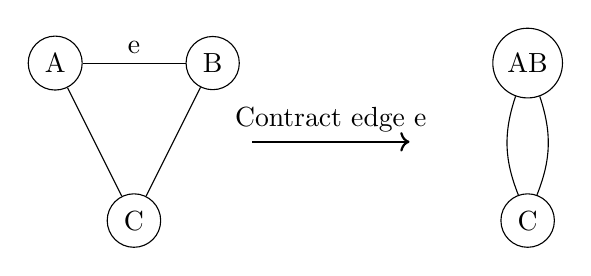
\begin{tikzpicture}
        \node[draw, circle] (A) at (0, 1) {A};
        \node[draw, circle] (B) at (2, 1) {B};
        \node[draw, circle] (C) at (1, -1) {C};
    
        \draw (A) -- (B) node[midway, above] {e};
        \draw (B) -- (C);
        \draw (A) -- (C);
    
        \draw[->, thick] (2.5, 0) -- (4.5, 0) node[midway, above] {Contract edge e};
    
        \node[draw, circle] (AB) at (6, 1) {AB};
        \node[draw, circle] (C2) at (6, -1) {C};

        \draw (AB) to [bend left=20] (C2);
        \draw (AB) to [bend right=20] (C2);
    \end{tikzpicture}
\end{center}
\noindent Each contraction reduces the number of vertices by 1, and we want to stop when we have two vertices left. This leaves us with two vertices and many edges between them.
\nt{We allow multi-edges.}
\noindent \textbf{Question:} Should we keep self-edges?

\noindent \textbf{Answer:} No. Delete them.

\noindent The observation we make is that we win iff edges at the end are a min-cut.

\subsection{Karger's Algorithm}
\noindent The algorithm is as follows:
\begin{itemize}
    \item Randomly pick an edge $(u, v)$.
    \item Contract $(u, v)$.
    \item Repeat until 2 vertices are left.
\end{itemize}
\mlenma{}{For any min-cut C, the probability that Karger's algorithm finds C is $\geq \frac{1}{\text{poly}(n)}$.}
\begin{proof}
    Let $e_1, e_2, \ldots$ be the edges we contract. Let's start by considering $P(e_1 \in C)$.

    We first have $P(e_1 \in C) = \frac{|C|}{|E|}$, but there's something better to notice. Let $d$ be the minimum degree of any vertex in $G$. Then $|C| \leq d$ and $|E| \geq \frac{dn}{2}$. So $P(e_1 \in C) \leq \frac{2}{n}$ and $P(e_1 \notin C) \geq 1 - \frac{2}{n}$.

    Now consider $P(e_2 \notin C \mid e_1 \notin C)$. By the same analysis, we have $P(e_2 \notin C \mid e_1 \notin C) \geq 1- \frac{2}{n-1}$. This is because after we contract $e_1$, we have $n-1$ vertices left. So, $C$ is still a min-cut with respect to the remaining vertices. Set $d$ as the new minimum degree, and we have $|C| \leq d$ and $|\text{remaining edges}| \geq \frac{d(n-1)}{2}$. Then:
    \begin{align*}
        P(e_2 \in C \mid e_1 \notin C) = \frac{|C|}{|\text{remaining edges}|} \leq \frac{d}{\frac{d(n-1)}{2}} = \frac{2}{n-1}.
    \end{align*}
    Now:
    \begin{align*}
        P(e_3 \notin C | e_1, e_2 \notin C) &\geq 1 - \frac{2}{n-2} \\
        &\vdots \\
        P(e_k \notin C | e_1, \ldots, e_{k-1} \notin C) &\geq 1 - \frac{2}{n-k+1}.
    \end{align*}
    So,
    \begin{align*}
        P(\text{we find } C) = P(e_1, \ldots, e_{n-2} \notin C) &\geq \left(\frac{n-2}{n}\right) \left(\frac{n-3}{n-1}\right) \ldots \left(\frac{1}{3}\right) \\
        &\approx \frac{2}{n(n-1)}.
    \end{align*}
\end{proof}
\textbf{Conclusion:} The algorithm succeeds with probability $\geq  \frac{2}{n(n-1)}$.

\noindent \textbf{New Goal:} Find min-cut with $\geq 1 - \frac{1}{n^2}$ probability. 

\noindent \textbf{Idea:} Repeat $t$ times and return the best cut we find. (We will determine the value for $t$ below.)

The probability that all $t$ trials fail is $\leq \left(1 - \frac{2}{n(n-1)}\right)^t$. We want this to be $\leq \frac{1}{n^2}$. We utilize the inequality below:
\begin{align*}
    \left(1 - \frac 1k\right)^k \leq \frac 1e \leq \left( 1 - \frac 1k\right)^{k-1}.
\end{align*}
So,
\begin{align*}
    \left(1 - \frac{2}{n(n-1)}\right)^t &\leq \frac{1}{e^{t \cdot \frac{2}{n(n-1)}}}\implies t = 2\binom n2 \log n \\
    &\leq \frac{1}{e^{2\log n}} = \frac 1{n^2},
\end{align*}
as desired. 
\subsection{Karger-Stein Algorithm}
We start with the following motivation. We have:
\begin{align*}
    P(\text{first }n/2 \text{ contractions succeed}) \geq \frac{n-2}{n} \frac{n-3}{n-1} \ldots \frac{n/2 - 1}{n/2 + 1} \approx \frac{1}{4}.
\end{align*}
This is because after we telescope, the bottom two terms are both near $n$ while the top two terms are near $n/2$. So now, if the first $n/2$ contractions succeed, what's the probability that the next $n/4$ succeed?
\begin{align*}
    P(\text{next }n/4 \text{ contractions succeed}) \geq \frac{n/2 - 2}{n/2} \frac{n/2 - 3}{n/2 - 1} \ldots \frac{n/4 - 1}{n/4 + 1} \approx \frac{1}{4}.
\end{align*}
And this pattern continues. 
\newpage \noindent We now go over the Karger-Stein algorithm:
\begin{itemize}
    \item Represent the problem as a tree.
    \item For the first $n/2$ contractions, run Karger's algorithm 4 times.
    \item For the next $n/4$ contractions, run Karger's algorithm 16 times.
    \item So on, until the base case of the algorithm which is when there are two vertices left. 
\end{itemize}


\begin{center}
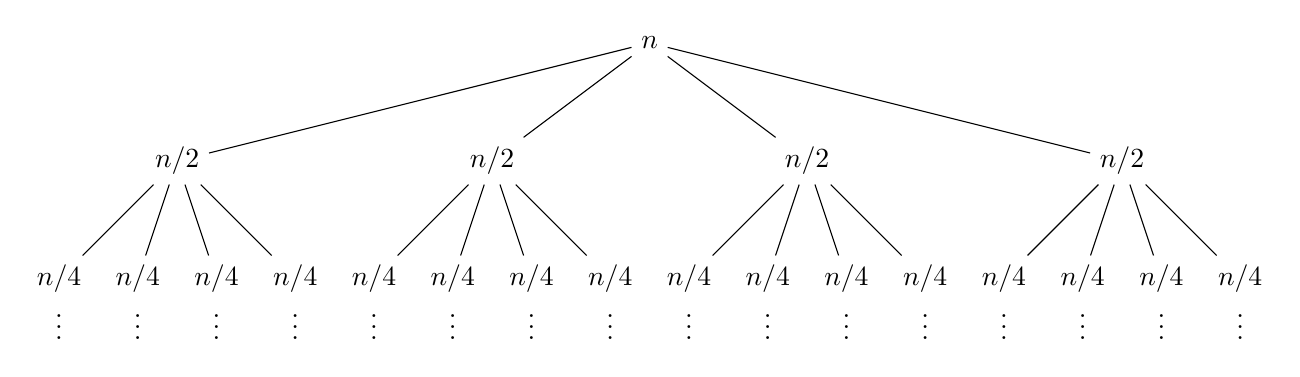
\begin{tikzpicture}[
    level distance=1.5cm,
    level 1/.style={sibling distance=4cm},
    level 2/.style={sibling distance=1cm},
    ]
    
    \node {$n$} % Root node
      child {node {$n/2$}
        child {node {$n/4$}
          child [level distance=0.25cm] {edge from parent[draw=none] child {node {$\vdots$} edge from parent[draw=none]}}
        }
        child {node {$n/4$}
          child [level distance=0.25cm] {edge from parent[draw=none] child {node {$\vdots$} edge from parent[draw=none]}}
        }
        child {node {$n/4$}
          child [level distance=0.25cm] {edge from parent[draw=none] child {node {$\vdots$} edge from parent[draw=none]}}
        }
        child {node {$n/4$}
          child [level distance=0.25cm] {edge from parent[draw=none] child {node {$\vdots$} edge from parent[draw=none]}}
        }
      }
      child {node {$n/2$}
        child {node {$n/4$}
          child [level distance=0.25cm] {edge from parent[draw=none] child {node {$\vdots$} edge from parent[draw=none]}}
        }
        child {node {$n/4$}
          child [level distance=0.25cm] {edge from parent[draw=none] child {node {$\vdots$} edge from parent[draw=none]}}
        }
        child {node {$n/4$}
          child [level distance=0.25cm] {edge from parent[draw=none] child {node {$\vdots$} edge from parent[draw=none]}}
        }
        child {node {$n/4$}
          child [level distance=0.25cm] {edge from parent[draw=none] child {node {$\vdots$} edge from parent[draw=none]}}
        }
      }
      child {node {$n/2$}
        child {node {$n/4$}
          child [level distance=0.25cm] {edge from parent[draw=none] child {node {$\vdots$} edge from parent[draw=none]}}
        }
        child {node {$n/4$}
          child [level distance=0.25cm] {edge from parent[draw=none] child {node {$\vdots$} edge from parent[draw=none]}}
        }
        child {node {$n/4$}
          child [level distance=0.25cm] {edge from parent[draw=none] child {node {$\vdots$} edge from parent[draw=none]}}
        }
        child {node {$n/4$}
          child [level distance=0.25cm] {edge from parent[draw=none] child {node {$\vdots$} edge from parent[draw=none]}}
        }
      }
      child {node {$n/2$}
        child {node {$n/4$}
          child [level distance=0.25cm] {edge from parent[draw=none] child {node {$\vdots$} edge from parent[draw=none]}}
        }
        child {node {$n/4$}
          child [level distance=0.25cm] {edge from parent[draw=none] child {node {$\vdots$} edge from parent[draw=none]}}
        }
        child {node {$n/4$}
          child [level distance=0.25cm] {edge from parent[draw=none] child {node {$\vdots$} edge from parent[draw=none]}}
        }
        child {node {$n/4$}
          child [level distance=0.25cm] {edge from parent[draw=none] child {node {$\vdots$} edge from parent[draw=none]}}
        }
      };
\end{tikzpicture}
\end{center}

\noindent \textbf{Time Analysis}: The first level takes $\tilde{O}(n^2)$ time. The second level takes $\tilde{O}\left(\frac{n^2}{2}\right)$ time. The third level takes $\tilde{O}\left(\frac{n^2}{4}\right)$ time. So the total time is $\tilde{O}(n^2)$. 

\noindent So, at level $i$:
\begin{itemize}
    \item There are $4^i$ edges.
    \item The work per edge $\leq (|\text{remaining vertices}|)^2 = \tilde{O}\left(\frac{n}{2^i}\right)^2 = \tilde{O}\left(\frac{n^2}{4^i}\right)$. 
\end{itemize}
This implies that the cost of the $i$th level is less than $\tilde O(n^2)$. Summing, we get a total cost $\tilde O(n^2)$.

Now we consider the probability that our algorithm succeeds. Again, we have a $4$-ary tree with a depth of $t = O(\log n)$. Each edge flips a coin where $P(\text{heads}) = \frac 14$. So what we want is a $t$ length chain of all heads. We can show the following result:
\begin{align*}
    P(\text{good path}) \geq \frac 1t \geq \Omega \left(\frac{1} {\log n}\right).
\end{align*}

The goal is an algorithm that succeeds with probability greater than $1 - \frac{1}{n^2}$. 

\noindent \textbf{Exercise:} $O(\log^2 n)$ repetitions suffice.

\section{Galton Walton Tree}
Building on the previous problem, we introduce the concept of a Galton Walton tree. This is a $4$-ary tree with $t$ levels where each edge flips a biased coin. The probability of heads is $1/4$. A root-to-leaf path in this tree is ``successful'' if all edges are heads.

\noindent \textbf{Claim:} $P(\text{successful path}) \geq \frac{1}{t}$.
\begin{proof}
    Pretend the paths are independent. Then we have that
    \begin{align*}
        P(\text{No successful path}) = \left(1 - \frac{1}{4^t}\right)^{4^t} \leq \frac{1}{e}.
    \end{align*}

    This is not a very interesting result. It is worth noting that the paths are extremely dependent on each other. Consider a path of length $t-2$ and creating two separate paths by diverging at the last edge. This should illustrate the dependence of the paths.

    Now let $f_t$ the probability of tailing in a tree with $t$ levels. We can define this as a recurrence on $f_{t-1}$. We have:
    \begin{align*}
        f_t = \left(\frac{1}{4} f_{t-1} + \frac{3}{4}\right)^4.
    \end{align*}

    To proceed with induction on $t$, we first prove the following identity:
    \begin{align*}
        1 - 1/k < \frac{1}{e^{1/k}} < 1 - 1/(k+1).
    \end{align*}
    This is a useful identity to have in our back pocket. We have:
    \begin{align*}
        (1 - 1/k)^k &< 1/e < (1 - 1/k)^{k-1} \\
        \implies 1 - 1/k &< 1/e^{1/k} \\ 1/e^{1/(k-1)} &< 1 - 1/k \implies 1/e^{1/k} < 1 - 1/(k+1).
    \end{align*}
    Putting it all together, we get the desired result. We can now proceed with induction.

    Our hypothesis: $f_{t-1} \leq 1 - \frac{1}{t-1}$. What we want to show is that $f_t \leq 1 - \frac 1t$. 

    We have:
    \begin{align*}
        f_t &\leq \left( \frac 34 + \frac 14 \left( 1 - \frac{1}{t-1} \right)\right)^4 \\
        &= \left(1 - \frac{1}{4(t-1)}\right)^4 \\
        &\leq \left(\frac{1}{e^{\frac{1}{4(t-1)}}}\right)^4 \\
        &= \frac{1}{e^{1/(t-1)}} \tag{by the above identity}\\
        &< 1 - \frac{1}{t}. \tag{by the above identity}
    \end{align*}
    This completes the induction, as well as the entire proof.
\end{proof}


\chapter{Lovasz Local Lemma}{}
\mlenma{Lovasz Local Lemma}{Let $A_1, A_2, \ldots, A_n$ be ``bad events.'' Suppose:
\begin{itemize}
    \item $P(A_i) < p$ for some $p$.
    \item Each $A_i$  has a ``dependency set'' $D_i \subseteq \{A_1, A_2, \ldots, A_n\}$ such that $A_i$ is independent of $\{A_1, A_2, \ldots, A_n\} \setminus D_i$ and $|D_i| \leq d$. 
\end{itemize}
If $p < \frac{1}{ed}$, then there exists an outcome where none of the $A_i$ occur. That is, $P(\text{no bad events}) \geq \frac{1}{d^n}$.}
\noindent \textbf{Application:} KSAT. In KSAT, we have a bunch of boolean variables $x_1, x_2, \ldots$. A K-SAT formula is a conjunction of $n$ clauses, where each clause selects $k$ unique variables that cannot take a specific form. For example, if we have $k=3$, we might have a clause that says $(x_1, x_2, x_3) \neq (0, 1, 0)$. The question is whether we can find a satisfying assignment of these variables. 

\thm{}{Suppose each clause overlaps in variables $\leq d-1$ other clauses. Also suppose $\frac{1}{2^k} < \frac{1}{ed}$. Then, there exists a satisfying assignment.}
\begin{proof}
    $x_1, x_2, \ldots$ are random $0, 1$ variables. Let $A_i$ be the event that clause $i$ is not satisfied. Then $P(A_i) \leq \frac{1}{2^k}$. By the LLL, there exists a satisfying assignment.
\end{proof}

\section{Algorithmic Lovasz Local Lemma}
\subsection{Algorithmic Setting}
We have random variables $X_1, X_2, \ldots, X_n$ and events $A_i$ that are determined by some subset of the $X_i$s. We can think about this as a dependency graph where all the $X_i$ and $A_i$ are nodes, and edges are drawn between $X_i$ and $A_j$ if $X_i$ determines $A_j$.

\mlenma{Algorithmic Lovasz Local Lemma}{Suppose each $A_i$ overlaps with at most $d-1$ other $A_j$s on which $X_i$s they use. Suppose $P(A_i) < \frac{1}{4d}$. Then there exists a polynomial time algorithm$^*$ that finds an outcome of $X_i$s such that none of the $A_i$s occur.}

\newpage
\subsection{Moser's Fix-it Algorithm}
% "i was going to present the proof from the paper, but a few days ago i came up with a much better proof". allegedly was a great proof solving a 30 year old open problem and slams it in 30 minutes. two weeks later, moser leaves academia and works in finance

\textbf{Algorithm:}
\begin{itemize}
    \item Sample $X_1, X_2, \ldots, X_m$.
    \item While $\exists$ bad event $A_i$:
    \begin{itemize}
        \item Pick $A_i$ arbitrarily.
        \item Resample the $X_i$'s that determine $A_i$.
    \end{itemize}
\end{itemize}

\thm{Moser's Theorem (KSAT)}{Consider KSAT:
\begin{itemize}
    \item $m$ vars, $X_1, \ldots, X_m$.
    \item $n$ clauses $C_1, \ldots, C_n$.
    \item Each $C_i$ depends on $\leq d$ other $C_i$'s. 
\end{itemize}
If $8d < 2^k$, then Moser's algorithm performs $t = O(n)$ (really $O \left( \frac nd \right)$) fix-its in expectation. }
\noindent \textbf{Proof Idea:}
Use random bits, for example $R=0010010100101\ldots$. Construct a ``transcript'' $T$ such that if you tell me $T$, I can recover all the random bits you used. The interesting property of $T$ is that:
\begin{align*}
    |T| \leq (\text{number of fix-its}) \cdot (2 \lg d) + O(n).
\end{align*}
The number of random bits we use is less than the number of fix-its times $k$. We know that $k > (2 + \lg d) \cdot 100$. 

If Moser's algorithm runs for a long time, say $> 100n$ fix-its, then
\begin{align*}
    |T| \leq 100n \cdot (2 \lg d) + O(n).
\end{align*}
Then,
\begin{align*}
    \text{number of random bits} &= 100n \cdot k \\
    &> 100n \cdot (2 + \lg d) \cdot 100.
\end{align*}
This means $|T| << \text{number of random bits}$. So if we can show that such a $T$ exists, then we can show that the expected number of fix-its to be pretty small.

\subsection{Proof of Moser's Theorem}
\begin{proof}
    We start by defining variables we are going to use:
    \begin{itemize}
        \item $R =$ random bits used by the algorithm. 
        \item $M_1 =$ final values of $X_i$'s. 
        \item $M_2 =$ sequence of which clauses we fix.
    \end{itemize}
    \mlenma{}{$M_1$ and $M_2$ fully determine $R$.}
    \begin{proof}
        Work backwards! Consider the last $C_i$ that was fixed. We know its variables after the fix and the variables before the fix. So we can ``undo'' the fix. We can keep doing this until we get to the beginning.
    \end{proof}
    \mlenma{}{$M_2$ can be compressed to $n + t(2 + \lg d)$ bits.}
    We'll proceed by assuming the lemma first. So now we have $|M_1| = m$ and $|R| = m + tk$. Also since $8d < 2^k$< we have $3 + \lg d \leq k$. So, $|R| \geq m + t(3 + \lg d)$. 

    Now,
    \begin{align*}
        |M_1| + |M_2| &= n + m + t(2 + \lg d) \\
        &\leq |R| + n - t.
    \end{align*}
    If $E[t] > n$, then $E[|M_1 \circ M_2|] < E[|R|]$. This is a contradiction by the incompressibility of random bits. So, $E[t] \leq n$ as desired.
\end{proof}

    \noindent Now we return to proving the second lemma. 
    \begin{proof}
    We start by defining processes.

    \noindent Define process($C_i$):
    \begin{itemize}
        \item Resample $C_i$'s variables.
        \item While $\exists$ another $C_j$ that is broken and depends on $C_i$:
        \begin{itemize}
            \item Select such a $C_j$.
            \item process($C_j$).
        \end{itemize}
    \end{itemize}


    \noindent Define Algorithm:
    \begin{itemize}
        \item For $i = 1, \ldots, n$:
        \begin{itemize}
            \item If $C_i$ is broken, process($C_i$).
        \end{itemize}
    \end{itemize}
    \textbf{Claim:} When the algorithm finishes, all clauses holds.

    \noindent \textbf{Claim:} Algorithm terminates with probability 1.

    \noindent We now look towards constructing $M_2$:
    \begin{itemize}
        \item $A =$ Part 1: $n$ bits, which $C_i$'s get fixed in for loop.
    \end{itemize}
    Now recall the process algorithm. Notice here that for each $C_j$, there are only $d+1$ options. This means that we can communicate $C_j$ with $\lg(d+1)$ bits, which we'll call $q$. We now rewrite process considering a string $B$.

    \noindent Define process($C_i$):
    \begin{itemize}
        \item Resample $C_i$'s variables.
        \item While $\exists$ another $C_j$ that is broken and depends on $C_i$:
        \begin{itemize}
            \item Select such a $C_j$.
            \item $B = B + ``1" + q$.
            \item process($C_j$).
        \end{itemize}
        \item $B = B + ``0"$.
    \end{itemize}
So given $M_2$, $A$ lets us recover which clauses the for loop fixes. $B$ lets us figure out which clauses are fixed within each process subroutine. This means we can recover the entire sequence of clause fixes that the algorithm performs.

So, $|A| = n$ and $|B| = t(2 + \lg d)$. This means $|A \circ B| = n + t(2 + \lg d)$, which completes the proof.
\end{proof} 


\chapter{Chernoff Bounds}
We start with an example. Suppose I flip 100 fair coins. What is the probability that the number of heads is greater than or equal to 75? Turns out,
\begin{align*}
    P(\text{heads} \geq 75) &\approx \frac{1}{3.5 \times 10^6}.
\end{align*}
\thm{}{
    Consider $n$ fair coin flips, $X_1, X_2, \ldots, X_n$ iid with $X_i = \begin{cases} 0 & \text{w.p. $1/2$} \\ 1 & \text{w.p. $1/2$} \end{cases}$. Let $X = \sum X_i$. Then,
    \begin{align*}
        P\left(X > \frac n2  + K \sqrt n\right) \leq e^{-\Omega(K^2)}.
    \end{align*}
}
\cor{}{
    \[P\left( X \geq \frac 34 n \right) \leq e^{-n/32}\]
}
\noindent You don't actually need $X_1, \ldots, X_n$ to be independent. It suffices to have that, for any $i$ and any outcomes of $X_1, \ldots, X_{i-1}$,
\begin{align*}
    P(X_i = 1 \mid X_1, \ldots, X_{i-1}) \leq 1/2.
\end{align*}
\nt{``Azuma's Inequality'' is a citable Chernoff bound. Alternatives include ``multiplicative version of Azuma's inequality'' and ``Freedman's inequality.''}
\noindent We turn to the proof of the theorem.
\begin{proof}
    Idea: suppose we have a function $f$ such that:
    \begin{itemize}
        \item $f$ is non-negative.
        \item $f$ is increasing on $[n/2, n]$.
    \end{itemize}
    Then, 
    \begin{align*}
        P\left(x \geq \frac  n2 + K \sqrt n\right) \leq P\left(f(x) \geq f\left(\frac n2 + K \sqrt n\right)\right) \leq \frac{E[f(x)]}{f\left(\frac n2 + K \sqrt n\right)}. 
    \end{align*}
    \ex{Trying $f$'s}{
        $f(x) = \left(x - \frac n2\right)^2$. This clearly satisfies the requirements. This tells us that:
        \begin{align*}
            P\left(x > \frac n2 + K \sqrt n\right) &\leq \frac{E[f(x)]}{K^2n} \\
            &= \frac{\Var(X)}{K^2n}.
        \end{align*}
        We use the linearity of variance. We have $\text{Var}(X_i) = \frac 14$. So, $\text{Var}(X) = \frac n4$. Thus,
        \begin{align*}
            P\left(x > \frac n2 + K \sqrt n\right) \leq \frac{1}{4k^2}.
        \end{align*}
        This is exactly Chebyshev's inequality.
    }
    \noindent We now find an $f$ that proves our result. Try $f(x) = e^{\lambda x}$ for some $\lambda \in (0, 1)$. This is approximately ${(1+\lambda)}^x$. We first find the expectation:
    \begin{align*}
        E[f(x)] = E[e^{\lambda \sum_i X_i}] &= E\left[\prod_i e^{\lambda X_i}\right] \\
        &= \prod_i E[e^{\lambda X_i}] \tag{by independence} \\
        &= \left( \frac{1 + e^\lambda}{2} \right)^n.
    \end{align*}
    \noindent \textbf{Fact:} \begin{align}
        e^\lambda &= 1 + \lambda + \frac{\lambda^2}{2!} + \frac{\lambda^3}{3!} + \cdots \\
        &\leq 1 + \lambda + \lambda^2 \cdot\left(\frac {1}{2!} + \frac {1}{3!} + \cdots \right) \\
        &\leq 1 + \lambda + \lambda^2.
    \end{align}
    It follows that
    \begin{align*}
        E[e^{\lambda X_i}] &\leq 1+ \frac 12 \lambda + \frac 12 \lambda^2.
    \end{align*}
    Now we make use of the other fact that $1 + x \leq e^x$. So
    \begin{align*}
        E[e^{\lambda X_i}] &\leq 1+ \frac 12 \lambda + \frac 12 \lambda^2 \\
        &\leq e^{\lambda/2 + \lambda^2/2}.
    \end{align*}
    Thus,
    \begin{align*}
        E[f(x)] &\leq e^{n(\lambda/2 + \lambda^2/2)}.
    \end{align*}
    So now,
\begin{align*}
    P\left(X > \frac n2 + K \sqrt n\right) &\leq \frac{E[f(x)]}{f\left(\frac n2 + K \sqrt n\right)} \\
    &\leq \frac{e^{n(\lambda/2 + \lambda^2/2)}}{e^{n\lambda/2 + \lambda K \sqrt n}} \\
    &= e^{n\lambda^2 / 2 - \lambda K \sqrt n}.
\end{align*}
Now we try to find an appropriate value for $\lambda$. We try:
\begin{align*}
    \lambda K \sqrt n &= n\lambda^2\\
    \frac{K}{\sqrt n} &= \lambda.
\end{align*}
This yields:
\begin{align*}
    e^{n\lambda^2 / 2 - \lambda K \sqrt n} &= e^{-\lambda K \sqrt  n /2} = e^{-k^2/2},
\end{align*}
as desired.
\end{proof}
\section{Quicksort Algorithm (1961)}
We review the algorithm for quicksort:
\begin{itemize}
    \item Pick random pivot $P$.
    \item Partition elements into 2 pieces: elements smaller/larger than $P$.
    \item Recurse on the pieces.
\end{itemize}
\thm{}{The running time of quicksort satisfies $T = O(n \lg n)$ with probably at least $1 - \frac{1}{n^2}$.}
\begin{proof}
    Note that the time is $\leq \#\text{levels} \cdot O(n)$. So what we have to prove is that with high probability, the depth of the algorithm doesn't exceed $\lg n$. So,
    \begin{align*}
        P(\text{max depth} \geq 1000\lg n) &\leq P(\exists \text{element with max depth} \geq 1000 \lg n) \\
        &\leq n \cdot P(\text{a given $v$ has depth} \geq 1000 \lg n).
    \end{align*}
    We want to show that the probability on the last line is $\leq \frac{1}{n^3}$. We have that
    \begin{align*}
        P(\text{next subproblem} \leq 3/4 \text{current size}) \geq \frac 12.
    \end{align*}
    Let $P_1, P_2, \ldots$ be subproblems in $v$'s path. Let 
    \begin{align*}
        X_i = \begin{cases}
            1 & P_{i+1} \text{exists and } |P_{i+1}| > \frac 34 |P_i| \\
            0 & \text{otherwise}
        \end{cases}
    \end{align*}
    We observe that $P(X_i = 1 \mid X_1, \ldots, X_{i-1}) \leq 1/2$. So by Chernoff bound, if we look at $X = X_1 + X_2  + \cdots + X_{1000 \lg n =: m}$, we get:
    \begin{align*}
        P\left( X \geq \frac 34 m\right) \leq e^{-m/32} <<< \frac{1}{n^3}.
    \end{align*}
    If $X \leq \frac 34 m$, either $P_m$ doesn't exist or $|P_m| \leq n \cdot \left( \frac 34 \right)^{m/4} = n \cdot \left( \frac 34 \right)^{250 \log n} << 1$, which is a contradiction. This means $P_m$ in fact does not exist. As such, we are able to conclude that we have a running time of $O(n \lg n)$ with the desired probability.
\end{proof}

\newpage
\section{Revisiting Theorem 4.0.1}
We start with warm-ups to give an alternative proof to Theorem 4.0.1.

\subsection{Poor Man's Chernoff Bound}
\thm{}{\[P(X \geq 2K\sqrt n) \leq \frac{1}{2^K}.\]}
\begin{proof} We make use of the core facts below:

    \noindent\textbf{Core fact 1}: $P(X \geq 2\sqrt n) \leq \frac{1}{4}$, by Chebyshev's inequality.

    \noindent\textbf{Core fact 1'}: $P($any prefix has sum $\geq 2 \sqrt n) \leq \frac 12$. This is a direct result of \textbf{Core fact 1}, and the implication will be shown in the homework. 
    
    We can graph the running sum as a function of time and track the times that we hit the values $2\sqrt n$, $4 \sqrt n$, and $6\sqrt n$ and call them $t_1, t_2, t_3,$ et cetera. What the core fact is saying is that $P(t_1$ exists$) \leq \frac 12$. Then, we can build the the following chain:
    \begin{align*}
        P(t_1 \text{ exists}) &\leq \frac 12 \\
        P(t_2 \text{ exists} \mid t_1 \text{ exists}) &\leq \frac 12 \\
        &\vdots \\
        P(t_i \text{ exists} \mid t_{i-1} \text{ exists}) &\leq \frac 12.
    \end{align*}
    So, 
    \begin{align*}
        P(X \geq 2K \sqrt n) \leq P(t_K \text{ exists}) \leq \frac{1}{2^K},
    \end{align*}
    as desired.
\end{proof}

\subsection{Chernoff Bound for Geometric Random Variables}
\thm{}{Let $X_1, \ldots, X_n$ be non-negative independent random variables such that for all $j \in \NN$,
\begin{align*}
    P(X_i \geq j) \leq p^j.
\end{align*}
Then $X = \sum X_i$ satisfies
\begin{align*}
    P(X \geq 2n) \leq (4p)^n.
\end{align*}
}
\begin{proof}
    $X \geq 2n \implies \sum \lfloor X_i \rfloor \geq n \implies \exists \langle Y_1, \ldots, Y_n\rangle =: \vec Y$ such that 
    \begin{itemize}
        \item $\sum Y_i  = n$.
        \item $X_i \geq Y_i \, \forall i$. 
    \end{itemize}
    For a given option $\langle Y_1, \ldots, Y_n\rangle$ for $\vec Y$,
    \begin{align*}
        P(\vec Y \text{ occurs}) &= P(X_i \geq Y_i \forall i) \\
        &\leq \prod_{i} P(X_i \geq Y_i) \\
        &\leq \prod_i p^{Y_i} \\
        &= p^{\sum_i Y_i} \\
        &= p^n.
    \end{align*}
    Now we bound the number of options for $\vec Y$. We can express $\vec Y$ as a binary string, for example:
    \begin{align*}
        \underbrace{000}_{Y_1 = 3}1\underbrace{0}_{Y_2=1} 1\underbrace{}_{Y_3 = 0}1 \ldots   
    \end{align*}
    So the number of $0$'s is $\sum Y_i = n$ and the number of $1$'s is $n$. This means that the number o options satisfying $\sum Y_i = n$ is less than the number of binary strings of length $2n$ which is $4^n$. 

    So,
    \begin{align*}
        P(X \geq 2n) \leq P(\text{some } \vec Y \text{ occurs}) \\
        &\leq (\text{\# of options for } \vec Y) \cdot P(\vec Y \text{ occurs}) \\
        &\leq 4^n \cdot p^n \\
        &= (4p)^n.
    \end{align*}
\end{proof}




\subsection{Anti-(Chernoff Bound)}
\thm{}{
\begin{align*}
    P\left(X \geq \frac K4 \sqrt n\right) \geq \frac{1}{4^{K^2}}
\end{align*}
}

\begin{proof}
    Break the coins into $K^2$ groups. So each group has $m = \frac{n}{K^2}$ coins. 

    \noindent \textbf{Core fact}: $P\left( X \geq \frac 14 \sqrt n\right) \geq \frac 14$.
    
    Let $C_i$ be the sum of the $i$-th group. So by the core fact, 
    \begin{align*}
        P\left(C_i \geq \frac 14 \sqrt m\right) \geq \frac 14.
    \end{align*}
    So,
    \begin{align*}
        P\left(\text{every } C_i \geq \frac 14 \sqrt m\right) \geq \frac{1}{4^{K^2}}
    \end{align*}
    If this occurs, then 
    \begin{align*}
        X = \sum C_i \geq K^2 \cdot\left(\frac 14 \sqrt m\right) = \frac K4 \sqrt n.
    \end{align*}
\end{proof}
\newpage 
\subsection{Real Chernoff Bound}
\thm{}{
    \begin{align*}
        P(X \geq 16k \sqrt n) \leq \frac{1}{2^{K^2}}.
    \end{align*}
}
\begin{proof}
    We start by defining $Y_i = \max\left(0, \frac{C_i}{8\sqrt m}\right)$. We can apply the Poor Man's Chernoff bound to each $C_i$ to get
    \begin{align*}
        P(C_i \geq 2\ell \sqrt m) &\leq \frac{1}{2^\ell} \\
        \implies P\left(Y_i \geq \frac{2\ell \sqrt m}{8\sqrt m}\right) &\leq \frac{1}{2^{\ell}} \\
        \implies P(Y_i \geq \ell) & \leq \frac{1}{2^{4\ell}} \leq \frac{1}{16^\ell}.
    \end{align*}
    This is saying that $Y_i$ are geometric random variables. So by the geometric random variable bound,
    \begin{align*}
        P\left(\sum Y_i \geq 2 K^2\right) \leq (4 \cdot 1/16)^{K^2} = \left(\frac 14 \right)^{K^2}.
    \end{align*}
    But also 
    \begin{align*}
        X \geq 16K \sqrt n &\implies \sum C_i \geq 16K \sqrt n \\
        &\implies \sum Y_i \geq \frac{16K \sqrt n}{8 \sqrt m} = 2K^2.
    \end{align*}
\end{proof}


\thm{}{
    Let $X_1, X_2, \ldots, X_n$ be independent $\{0, 1\}$ coin flips with $P(X_i = 1) = p$ for some $p \leq \frac 12$. Define $X = \sum X_i$, $\mu = E[X] = np$. 

    Small-deviation regime: For $K \in \{1, \ldots, \sqrt \mu\}$,
    \begin{align*}
        P(X \geq \mu + K\sqrt \mu) \leq e^{-\Theta(K^2)}. 
    \end{align*}
    Large-deviation regime: For $J \geq 2$ such that $J\mu \leq n$, 
    \begin{align*}
        P(X \geq J\mu) \leq \frac{1}{J^{\Theta(J \mu)}}.
    \end{align*}
}
\begin{proof}
    (large-deviation case)

    \noindent \underline{\textbf{Warmup 1}}
    \newline \newline
    \noindent \textbf{Theorem 1} (Poor Man's Chernoff Bound)
        If $\mu \leq 1$, then
        \begin{align*}
            P( X \geq K) \leq \mu^K.
        \end{align*}
    \begin{proof}
        \textbf{Core fact} $P(X \geq 1) \leq \mu$ by Markov's inequality. 

        Now repeat the ideas with $t_1, t_2, \ldots$ to say that $P(X \text{ reaches } i) = \mu^i$. 
    \end{proof}
    \newpage
    \noindent \underline{\textbf{Warmup 2}} This was already done prior as it is the exact same.
    \newline \newline
    \noindent \underline{\textbf{Warmup 3}}
    \newline \newline
    \noindent \textbf{Theorem 3}
    \begin{align*}
        P(X \geq J) \geq \frac{1}{J^{O(J\mu)}}
    \end{align*}
    \begin{proof}
        We'll have $J \mu$ groups where each group has mean $\frac 1J$. 

        \noindent \textbf{Core fact}: If $\mu \leq 1$, then $P(X \geq 1) \geq \Omega(\mu)$. 

        By the core fact, each $C_i$ is $\geq 1$ with probability $\geq \Omega \left( \frac 1J\right)$. So, 
        \begin{align*}
            P(\text{every } C_i \geq 1) = P(X \geq J\mu) \geq \Omega \left(\frac 1J\right)^{J \mu}.
        \end{align*}
        ``Squiggly square to signify almost proof done.''
    \end{proof}

    So the Poor Man's Chernoff Bound implies $P(C_i \geq K) \leq \frac{1}{J^K}$. Then by Chernoff for geometric random variables,
    \begin{align*}
        P\left(\sum C_i \geq 2J \mu\right) \leq \left(\frac{4}{J}\right)^{J \mu}
    \end{align*}

\end{proof}



\section{More Chernoff Bounds}
\thm{Chernoff Bound}{
    Let $X_1, X_2, \ldots, X_n \in [0, 1]$ be independent random variables. Let $X = \sum X_i$ and $\mu = E[X]$. Then, for $k \in O(\sqrt \mu)$, 
    \begin{align*}
        P(|X - \mu| \geq k \sqrt{\mu}) \leq e^{-\Omega(k^2)}.
    \end{align*}
    And for $J \geq 2$,
    \begin{align*}
        P(X \geq J\mu) \leq \left( \frac 1 J\right)^{\Omega(J\mu)}.
    \end{align*}
}
\noindent Small-deviation regime:
\begin{itemize}
    \item There are $k^2$ chunks.
    \item So each has expected value $\approx \frac{\mu}{k^2}$.
    \item If each exceeds expected value by $\sqrt{\frac{\mu}{k^2}}$, then the total sum is $\geq k^2 \cdot \sqrt{\frac{\mu}{k^2}} = k \sqrt \mu$. 
\end{itemize}
\noindent Large-deviation regime:
\begin{itemize}
    \item $J \mu$ chunks.
    \item Each chunk has expected value $\approx \frac 1J$.
    \item If each chunk is at least 1, then the total sum is at least $J \mu$. 
\end{itemize}
\thm{Bennett's Inequality, Bernstein's Bound}{
    Same bound, but let $v = \Var(X)$. 
    \begin{align*}
        P(X - E[X] \geq k\sqrt v) &\leq e^{-\Theta(k^)} \text{ for } k \in \{1, 2, \ldots, \sqrt v\} \\
        P(X - E[X] \geq Jv) &\leq \left( \frac 1J \right)^{\Omega(Jv)} \text{ for } J \geq 2.
    \end{align*}
}

\subsection{Adaptive Version}
\thm{Azuma's Inequality}{
    Let $X_1, X_2, \ldots, X_n \in [-1, 1]$. Suppose $E[X_i | X_1, \ldots, X_{i-1}] = 0$. Then, $X = \sum X_i$ satisfies
    \begin{align*}
        P(X \geq K\sqrt n) \leq e^{-\Omega(K^2)}.
    \end{align*}
}
\noindent Fancier versions:

Have random variables $X_1, X_2, \ldots, X_n \in [0, 1]$ which are revealed one after the other. After $X_1, \ldots, X_{i-1}$ are revealed, Alice gets to select the distribution $P_i$ for $X_i$ and then $X_i$ is revealed from $P_i$. 

Let $\mu_i = E[X_i \mid P_i]$, $v_i = \Var(X_i \mid P_i)$, $X = \sum X_i$, $\mu = \sum \mu_i$ and $v = \sum v_i$. As a corollary to Azuma's inequality,
\begin{align*}
    P( X \geq \mu + k \sqrt n) \leq e^{-\Omega(k^2)}.
\end{align*}

Now if $\mu$ is deterministically at most $\bar \mu$, then
\begin{align*}
    P(X \geq K \sqrt{\bar \mu} + \bar \mu) &\leq e^{-\Omega(K^2)} \\
    P(X \geq J \bar\mu) &\leq \left( \frac 1J \right)^{\Omega(J\bar \mu)}.
\end{align*}

\thm{Freedman's Inequality}{
    If $v$ is deterministcally at most $\bar v$, then
    \begin{align*}
        P(X \geq K \sqrt{\bar v} + \mu) &\leq e^{-\Omega(K^2)} \text{ for } K \in \{1, 2, \ldots, \sqrt v\} \\
        P(X \geq \mu + J \bar v) &\leq \left( \frac 1J \right)^{\Omega(J\bar v)} \text{ for } J \geq 2.
    \end{align*}
}   


\nt{Bill has used the following bound in $\sim 90 \%$ of his papers. 

``Sometimes when you don't need this bound you want to find a way to use it anyway.''}
\thm{McDiarmid's Inequality}{
    Let $X_1, X_2, \ldots X_n$ be independent. Let $F : X_1, \ldots, X_n \to \RR$. Suppose: If I change some $X_i$ to a new value $\bar X_i$,
    \begin{align*}
        |F(X_1, \ldots, X_i, \ldots, X_n) - F(X_1, \ldots, \bar X_i, \ldots, X_n)| \leq 1.
    \end{align*}
    Then, 
    \begin{align*}
        P(|F - E[F]| \geq K\sqrt n) \leq e^{-\Omega(K^2)}.
    \end{align*}
}

\ex{}{
    Consider a random graph:
    \begin{itemize}
        \item $n$ vertices.
        \item each $(i, j)$ is an edge with probability $\frac 12$.
    \end{itemize}
    Consider the chromatic number $\chi(G)$. There's a way to show that
    \begin{align*}
        P(|\chi(G) - E[\chi(G)] | \geq k \sqrt n) \leq e^{-\Omega(k^2)}.
    \end{align*}
    We cannot define the random variables $X_i$ on whether an edge is included or not. This is because we end up getting $n^2$ random variables, which makes the inequality flop. We proceed by defining $X_1, X_2, \ldots, X_n$ where $X_i$ is the number of edges from vertex $i$ to vertices $ > i$. Then the result follows directly from McDiarmid's inequality.
}
\noindent \textit{Proof Idea}: Let 
\begin{align*}
    Y_0 &= E[F] \\
    Y_1 &= E[F \mid X_1] \\
    Y_2 &= E[F \mid X_1, X_2] \\
    \vdots \\
    Y_n &= E[F \mid X_1, \ldots, X_n] = F.
\end{align*}
Then let 
\begin{align*}
    Z_1 = Y_1 - Y_0 \\
    Z_2 = Y_2 - Y_1 \\
    \vdots \\
    Z_n = Y_n - Y_{n-1}.
\end{align*}
\noindent Claim 1:  $E[Z_i \mid Z_1, \ldots, Z_{i-1}] = 0$. 

\noindent Claim 2: $|Z_i| \leq 1$. 

So by Azuma, $P(\sum Z_i > K \sqrt n) \leq e^{-\Omega(K^2)}$. But $\sum Z_i = Y_n - Y_0 = F - E[F]$. 


\chapter{Oblivious Routing}
We start with an $n$-node hypercube:
\begin{itemize}
    \item $n$ vertices: $1, \ldots n$.
    \item edges: For each pair $i,j$ if $i,j$ differ in exactly one bit, then we have edges $(i, j)$ and $(j, i)$. 
\end{itemize}
This graph contains $n \log n$ edges. Each vertex $i$ wants to send a message to another vertex $\pi(i)$, where $\pi$ is a permutation. Each edge can only send 1 message per time step (may have to wait in queue before goign down edge). 

\noindent Goal: Complete all the message sending within time $O(\log n)$.

\noindent Oblivious Routing: Each message decides its path at the beginning of time. 

\thm{Brebner, Valiant (Leslie) (1981)}{
    With probability $\geq 1 - \frac{1}{n^{1000}}$, we can achieve $O(\log n)$ total time. 
}
\begin{proof}
    Algorithm:
    \begin{itemize}
        \item To send $i \to \pi(i)$; 
        \begin{itemize}
            \item Pick random $r_i \in \{1, \ldots, n\}$.
            \item Phase 1: Send $i \to r_i$.
            \item Phase 2: Send $r_i \to \pi(i)$.
        \end{itemize}
    \end{itemize}
    We wait until a preplanned time to begin phase 2. To send $i \to r_i$, use bit-fixing where we fix bits from left to right. Let $u_i :=$ message going from $i \to r_i$, $P_i=$ path that $u_i$ takes. Focus on a fixed $i$. 

    \noindent Claim: With high probability, $u_i$ completes $p_i$ within $O(\log n)$ time. 

    \mlenma{Lemma 1}{
        If $i \neq j$, then edges in $P_i \cap P_j$ form a continguous subpath.
    }
    \begin{proof}
        Consider an edge in $P_i$. For example if we have
        \begin{align*}
            010111011001 \\
            010111111001
        \end{align*}
        we can say that the 011001 agrees with $i$ and $j$, while the 0101111 agrees with $r_i$ and $r_j$. 

        The values of $k$ where paths agree,
        \begin{align*}
            \{ k \mid r_i, r_j \text{ agree first $k$ bits}\} \cap \{k \mid i, j \text{ agree on final $n-k+1$ bits}\}.
        \end{align*}
        Note that the first set is a prefix of $1, \ldots n$ and the second set is a suffix of $1, \ldots n$. Therefore, their intersection is a continguous interval. 
    \end{proof}
    \mlenma{Lemma 2}{
        The number of time steps that $u_i$ spends in queues is at most $|S_i|$, where $S_i = \{ j \neq i \mid P_i \cap P_j \neq \emptyset\}$.
    }
    \begin{proof}
        Say that a message $w$ that is currently on $P_i$ has ``delay'' $d$ if 
        \begin{itemize}
            \item $w$ is on the $t$-th step of $P_i$ for some $t$. 
            \item We are in the $t+d$-th time step of the algorithm.
        \end{itemize}
        If $u_i$ waits in a queue and its delay goes from $d$ to $d+1$, give a note with the number $d$ on it to whoever used the edge that $u_i$ wanted to use. Later on, if a message has a note ``$d$'', and $w$ waits in a queue:
        \begin{itemize}
            \item if edge $\notin P_i$, keep the note
            \item otherwise, pass the note to message that's using the edge we're waiting on.
        \end{itemize}
        If note $d$ is currently held by a message $w$ and if $w$ is still on $P_i$, then $w$'s delay is exactly $d$. This means that no two notes will be held by the same message. This implies that the number of notes is equal to the number of messages hold notes, which is then less or equal to $|S_i|$.
    \end{proof}
    Now let $e$ be an edge. Define $m_e :=$ the number of messages tha tuse $e$.
    \mlenma{Lemma 3}{
        $E[m_e] \leq 1$.
    }
    \begin{proof}
        What does it mean to use edge $e$? The first $k$ bits are free variables for $j$ while the last $n-k + 1$ agree with $j$. So the number of options for $j = 2^{k-1}$. FOr each such $j$, 
        \begin{align*}
            P(r_j \text{ has correct first $k$ bits}) = \frac{1}{2^k}.
        \end{align*}
        So,
        \begin{align*}
            E[\text{\# $j$ that use $e$}] \leq \sum_{\text{valid } j} P(\text{$j$ uses $e$}) \leq 2^{k-1} \frac{1}{2^k} = \frac 12.
        \end{align*}
    \end{proof}

    \mlenma{Lemma 4}{
        With high probability, $|S_i| \leq O(\log n)$.
    }
    \begin{proof}
        First, fix $P_i$. 
        \begin{align*}
            |S_i| = \sum_{j \neq i} \mathbb I [P_i \cap P_j \neq \emptyset],
        \end{align*}
        where $\mathbb I$ is the indicator function. Note that these are all independent random variables determined by $r_j$. This is exactly the type of thing we want to apply Chernoff bounds to. 

        Define $\mu := E[|S_i|] \leq \sum_{e \in P_i} E[\text{\# messages $j\neq i$ that use $e$}] \leq \frac{\log n}{2}$. 
    \end{proof}
    So let's say $\mu = \frac{\log n}{2}$. So,
    \begin{align*}
        P(|S_i| \geq J\mu) \leq \left( \frac 1J \right)^{\Omega(J\mu)} \leq \frac 12^{\Omega(J \mu)} \leq \frac{1}{\poly n}.
    \end{align*}
\end{proof}
\newpage 
\noindent Suppose I flip a fair coin repeatedly:

\noindent Question 1: How many flips do I need to get $\geq 1$ heads with high probability. 

\noindent Answer: $O(\log n) \implies P(\text{all tails}) \leq \frac{1}{2^{\Theta (\log n)}}$.

\noindent Question 2: How man flips do I need to get $\geq \log n$ heads with high probability?

\noindent Answer: $O(\log n)$. If I flip $1000 \log n$ coins, $P(\text{$< \log n$ heads}) = P(> 999 \log n \text{ tails})$. This means I exceeded the mean greatly as $E[\text{\# of tails}] = 500 \log n$. If $\mu = E[T]$, then
\begin{align*}
    T &> 1.9 \mu \\
    &> \mu + 0.9 \sqrt \mu ( \sqrt \mu).
\end{align*}
And the probability of this is $\leq e^{-\Omega(\log n)}$.

\chapter{Metric Embeddings}
\dfn{Metric Space}{
    A metric space $X$ is a set equipped with a function $d: X \times X \to \RR$ such that 
    \begin{enumerate}
        \item $d(x, y) \geq 0$ for all $x, y \in X$, $d(x,y) = 0$ if and only if $x = y$.
        \item $d(x,y) = d(y,x)$ for all $x,y \in X$
        \item $d(x,z) \leq d(x,y) + d(y, z)$ for all $x,y,z \in X$
    \end{enumerate}
}
\ex{}{
    \begin{itemize}
        \item $\ell^p$-distance. For $p \geq 1$, $X = \RR^k$. Then 
        \begin{align*}
            d_{\ell^p}(x, y) = \left( \sum_{i=1}^k |x_i - y_i|^p \right)^{1/p}. 
        \end{align*}
        \item Graph-distance. Take any undirected graph with positive weights, then you can talk about the graph distance between two vertices where 
        \begin{align*}
            d(v, u) = \text{graph distance}.
        \end{align*}
    \end{itemize}
}
\dfn{Metric Embeddings}{
    Given two metric spaces, $(X_1, d_1), (X_2, d_2)$, a map $\phi: X_1 \to X_2$ is a metric embedding with distortion at most $\alpha$ if $\exists \beta$ scaling parameter such that  $\forall x, y \in X_1$, $d_1(x, y)$ is within a factor of $\alpha$ of $\beta d_2(\phi(x), \phi(y))$. That is,
    \begin{align*}
        \beta d_2(\phi(x), \phi(y)) \leq d_1(x, y) \leq \alpha \beta d_2(\phi(x), \phi(y)).
    \end{align*}
}
\newpage 
\thm{Bourgain's Theorem}{
    Let $(X, d)$ be an $n$-point metric. Then there exists a function $\phi : (X; d) \to (\RR^{O(\log ^2 n)}, d_{\ell^1})$ such that the distortion is $O(\log n)$. 
}


\begin{proof}
    We review the algorithm. Let $c$ be a large constant. 
    \begin{itemize}
        \item For $i = 1, \ldots, \log n$,
        
        For $j = 1, \ldots, c \log n$,

        $S_{i, j} = \text{sample each element $x \in X$ with probability $2^{-i}$.}$
    \end{itemize}
\end{proof}

\mlenma{Key Lemma}{For $i \in \{1, \ldots, t\}$ and $j \in \{1, \ldots, c \log n\}$, we have with probability $\Omega(1)$ that 
\begin{align*}
    |d(x, S_{i, j}) - d(y S_{i, j})| \geq r_{i+1} - r_i.
\end{align*} }


I LEFT LECTURE HERE, FILLIN LATER 


\newpage
\section{Day 2}
\thm{}{Let $(X, d)$ be an $n$-point metric space. Suppose that $\forall x \neq y \in X$, $d(x, y) \in [1, n^2]$. We will embed $X$ into a tree metric $(T, d_T)$ with the following properties:
\begin{itemize}
    \item depth of tree is $O(\log n)$.
    \item For any root-leaf path, edge weights are decreasing powers of 2.
    \item Points in $X$ get mapped to leaves of the tree.
\end{itemize}
There exists a randomized embedding $\phi: X \to (T, d_T)$, where $T$ is also a random variable, such that 
\begin{itemize}
    \item $d_T(\phi(x), \phi(y)) \geq d(x, y)$.
    \item $E[d_T(\phi(x), \phi(y))] \leq O(\log n) d(x, y)$. 
\end{itemize}}
\begin{proof}
    The algorithm:
    \begin{enumerate}
        \item Pick a random permutation $\pi = \pi_1, \ldots, \pi_n$ of the elements of $X$.
        \item Pick uniformly random $\beta \in [1, 2]$. Define $\beta_i := 2^{i-1} \cdot \beta$.

        For each $x \in X$ and $i \in \{0, \ldots, 2\log n\}$, define 
        \begin{align*}
            \text{center}_i(x) = \text{first $\pi_j$ in permutation to satisfy $d(x, \pi_j) \leq \beta_i$}.
        \end{align*}
        \item Construct $\phi$ as follows:
        
        Each node represents a set of elements. Root at level $2\log n + 1 = $ all of $X$. For any node $w$ at level $i+1$, if node $>$ 1 element.
        \begin{itemize}
            \item Group $w$'s elements $z$ by $\text{center}_i(z) \to $ child nodes. 
        \end{itemize}
        Two elements $a, b \in w$ are in the same child iff $\text{center}_i(a) = \text{center}_i(b)$.
        \item Finally, edge from level $i+1$ to level $i$ has weight $2^{i}$. 
    \end{enumerate}
    Analysis:

    We first claim that for $x, y\in X$, $d_T(\phi(x), \phi(y)) \geq d(x, y)$. 
    \begin{proof}
        Observe that at level $i$, if $x,y$ in the same node, then $d(x, y) \leq 2\beta_i \leq 2^{i+1}$. So let $i$ be the highest level the path goes through, this implies that $d(x, y) \leq 2^{i+1}$. But also $d_T(\phi(x), \phi(y)) \geq 2\cdot 2^i \geq d(x, y)$ as desired.
    \end{proof}

    \mprop{}{\begin{align*}
        E[d_T(\phi(x), \phi(y))] \leq O(\log n) d(x, y).
    \end{align*}}
    \begin{proof}
        \begin{align*}
            d_T(\phi(x), \phi(y)) &\leq O(\text{largest edge weight along the path}) \\
            &\leq \sum_{i=0}^{2\log n} \mathbb I (\text{center}_i(x) \neq \text{center}_i(y)) \cdot 2^{i+1}.
        \end{align*}
        \newpage
        So we have 
        \begin{align*}
            E[d_T(\phi(x), \phi(y))] &\leq \sum_{i=0}^{2 \log n} \int_{r = 2^{i-1}}^{2^i} P(B_i = r) \cdot P(\text{center}_i(x) \neq \text{center}_i(y) \mid \beta_i = r) 2^{i+1} \text dr \\
            &=  \sum_{i=0}^{2 \log n} \int_{r = 2^{i-1}}^{2^i} \frac{1}{2^{i-1}} \cdot P(\text{center}_i(x) \neq \text{center}_i(y) \mid \beta_i = r) 2^{i+1} \text dr \\
            &=  \sum_{i=0}^{2 \log n} \int_{r = 2^{i-1}}^{2^i}  P(\text{center}_i(x) \neq \text{center}_i(y) \mid \beta_i = r) \text dr.
        \end{align*}
        If we look through $\pi_1, \pi_2, \ldots, \pi_n$, the first of $\{\text{center}_i(x), \text{center}_i(y)\}$ to appear is $w$ implies that $w$ ``cuts'' $(x, y)$ (and the centers are non-equal).

        Let $w_1, w_2, \ldots, w_n$ be elements of $x$ sorted by distance from $w_i$ to $\{x, y\}$. 

        \begin{align*}
            \sum_{i=0}^{2 \log n} \int_{r = 2^{i-1}}^{2^i}  P(\text{center}_i(x) \neq \text{center}_i(y) \mid \beta_i = r) \text dr &\leq \sum_{j=1}^n \sum_{i=0}^{2 \log n} \int_{r = 2^{i-1}}^{2_i} P(w \text{ cuts } (x, y) \mid \beta_i = r) \text dr.
        \end{align*}
        Call the integrand $\Xi$. We consider what must occur for $w_j$ to cut $(x, y)$. Suppose WLOG $d(w_j, x) \leq d(w_j, y)$. We need 
        \begin{itemize}
            \item $d(w_j, x) \leq \beta_i \leq d(w_j, y)$.
            \item $w_j$ must appear before $w_1, \ldots, w_{j-1}$ in $\pi$, which has probability $\leq \frac 1j$. 
        \end{itemize}
        So we get 
        \begin{align*}
            \sum_{j=1}^n \sum_{i=0}^{2 \log n} \int_{r = 2^{i-1}}^{2_i} P(w \text{ cuts } (x, y) \mid \beta_i = r) \text dr &\leq \sum_{j=1}^n \int_{z = d(w_j, x)}^{d(w_j, y)} \frac 1j \text dz \\
            &= \sum_{j=1}^n \frac 1j |d(w_j, y) - d_w(w_j, x)| \\
            &\leq d(x, y) \sum_{j=1}^n \frac 1j = d(x, y) O(\log n).
        \end{align*}
    \end{proof}
    
\end{proof}
\newpage
\section{Day 3}
\thm{Johnson-Lindenstrauss Lemma (1994)}{
    Let $\epsilon \in (0, 1)$. Let $S \subseteq \RR^d$ be a set of $n$ points. There exists a map $\phi : S \to \RR^{O(\log n) \cdot \epsilon^{-2}}$ which satisfies:
    \begin{align*}
        \forall a , b \in S, (1 \pm \epsilon)\Vert a- b \Vert_2 = \Vert \phi(a) - \phi(b) \Vert_2.
    \end{align*}
}
\noindent Our goal is to construct a linear $\phi$ such that for any $a \in \RR^d$, with high probability in $n$, 
\begin{align*}
    \Vert \phi (a) \Vert_2 = (1 \pm \epsilon) \Vert a \Vert_2. 
\end{align*}
If we can do this, then $\forall a, b \in S$, we have with high probability that
\begin{align*}
    \Vert \phi(a) - \phi(b) \Vert_2  &= \Vert \phi(a-b)\Vert_2 \\
    &= (1 \pm \epsilon) \Vert a- b \Vert_2.
\end{align*}
Then by applying the union bound over all $\binom n2$ pairs,  can complete the proof. 

\noindent We start with a warmup task. We want to construct a linear function $f: \RR^d \to \RR$ such that $E[f(a)^2] = \Vert a \Vert_2^2$. If we can find a function like this that also suffices:
\begin{align*}
    P(f(a)^2 > K\Vert a \Vert_2^2) \leq e^{-\Omega(K)},
\end{align*}
then we can finish the theorem off. 

\noindent \textbf{Review of normal random variables:} Let $v = $ variance, $\sigma  = \sqrt v$ (standard-deviation). Then $N(0, v)$ represents a normal random variable with mean 0 and standard deviation $\sigma$. 

\noindent \textbf{Fact 1:} Let $X \sim \mathrm N(0, \sigma^2)$. Then
\begin{align*}
    P(|X| \geq K \sigma) < 2e^{-K^2/3}.
\end{align*}

\noindent \textbf{Fact 2:} If $X \sim \mathrm(0, v_1)$ and $Y \sim \mathrm(0, v_2)$, and $X \perp Y$, then $X + Y \sim \mathrm(0, v_1 + v_2)$. 

\noindent \textbf{Fact 3:} Let $X \sim \mathrm N(0, v)$, $c \in \RR$. Then
\begin{align*}
    cX \sim \mathrm N(0, c^2v).
\end{align*}
For vector $\bar a = (a_1, \ldots, a_d)$, define 
\begin{align*}
    f(a) = \sum_{i=1}^d X_i \cdot a_i
\end{align*}
where $X_i$ is an independent random variable such that $X_i \sim \mathrm N(0, 1)$. That means $f(a) \sim \mathrm N(0, \Vert a \Vert_2^2)$. 

\cor{1}{$E[f(a)^2] = \Vert a \Vert_2^2$.}
\cor{2}{$P(f(a)^2 > K\Vert a \Vert_2^2) \leq e^{-\Omega(K)}$.}
\begin{proof}
    By the previous Chernoff bound,
    \begin{align*}
        P(|f(a)| > J \Vert a \Vert_2) &\leq e^{-J^2/3} \\
        P(f(a)^2 > J^2 \Vert a \Vert_2^2) &\leq 2e^{-J^2/3}.
    \end{align*}
    By setting $K = J^2$, we get the corollary.
\end{proof}
\newpage 
\noindent We now turn to the proof of the Johnson-Lindenstrauss lemma.
\begin{proof}
    Define $\phi(\vec a)$ as 
    \begin{align*}
        \phi(\vec a) = \langle \phi_1(\vec a), \ldots, \phi_r(\vec a)\rangle
    \end{align*}
    where $r = c\epsilon^{-2}\log n$ where $c$ is a large constant. Now we define $\phi_i$. We take the same argument as in the previous proof:
    \begin{align*}
        \phi_i(a) = \frac{1}{\sqrt r}\sum_{j=1}^d X_{i, j} \cdot a_j
    \end{align*}
    where all the $X_{i, j} \sim \mathrm N(0, 1)$ and are independent. We want to show:
    \begin{align*}
        \Vert \phi(\vec a) \Vert_2^2 &= (1 \pm \epsilon) \Vert a \Vert_2^2 \\
        \iff \sum \phi_i(\vec a)^2 &= (1 \pm \epsilon) \Vert a \Vert_2^2.
    \end{align*}
    We now go over a Chernoff bound for geometric random variables. Let $X_1, \ldots, X_n$ be independent. Let $\mu = E[\sum X_i]$. Suppose each $X_i$ satisfies 
    \begin{align*}
        P(|X_i| \geq K) \leq e^{-\Omega(k)}.
    \end{align*}
    Let $X = \sum X_i$. In the small-deviation regime ($K \in [1, \sqrt \mu]$), we have 
    \begin{align*}
        P(|X - E[X]| \geq K \sqrt{\mu}) \leq e^{-\Omega(k^2)}.
    \end{align*}
    Then for $J \geq 2$, we have 
    \begin{align*}
        P( X \geq J \mu) \leq \left( \frac 12 \right)^{\Omega(J\mu)}.
    \end{align*}
    Note that the large-deviation regime bound we're used to does not apply because it is not true in the $n=1$ case. Now for each $\phi_i$, we have 
    \begin{align*}
        r \cdot \phi_i(\vec a) \sim \mathrm N(0, \Vert a \Vert_2^2).
    \end{align*}
    If we wanted to normalize this, we would get 
    \begin{align*}
        Y_i := \left(\frac{\sqrt r \cdot \phi_i(\vec a)}{\Vert a \Vert_2}\right)^2 \sim \mathrm N(0, 1)^2.
    \end{align*}
    $Y_i$ has mean 1, and $|Y_i|$ is a geometric random variable. This means
    \begin{align*}
        P\left[\left| \sum_{i=1}^r Y_i - r \right| \geq K \sqrt r \right] \leq e^{-\Omega(k^2)}.
    \end{align*}
    Let's set $K\sqrt r = \epsilon r$, or that $K = \epsilon \sqrt r$. So,
    \begin{align*}
        P\left[\sum_{i=1}^r Y_i \neq (1 \pm \epsilon)r \right] = e^{-\Omega(\epsilon^2 r)}.
    \end{align*}
    But $-\Omega(\epsilon^2 r) = \frac{1}{\poly(n)}$. What follows is:
    \begin{align*}
        \sum \frac{r \phi_i(\vec a)^2}{\Vert a \Vert_2^2} &= (1 \pm \epsilon) r \\
        \implies \sum \phi_i(\vec a)^2 &= (1 \pm \epsilon) \Vert a \Vert_2^2.
    \end{align*}
    This is exactly what we wanted to prove. 
\end{proof}
\newpage
\noindent We now prove the facts about normal random variables. 
\cor{from Central Limit Theorem}{
    Suppoose you define $X^{(n)} := \sum_{i=1}^n X_i$ where $X_i$ takes on $1$ or $-1$ with probability $1/2$. Then as $n \to \infty$, $\frac {\sqrt v}{\sqrt n} X^{(n)}$ converges pointwise to a single distribution. This is the definition of $\mathrm N(0, v)$. 
}
\noindent As a shorthand, 
\begin{align*}
    \lim_{n\to\infty} \frac{\sqrt v}{n}X^{(n)} \sim N(0, v).
\end{align*}
We skip the first fact because it's an easy Chernoff bound. Fact 3 is also straight-forward from the definition of a random variable. So we will just prove that if we have $A, B\sim \mathrm N(0, v_1), \mathrm N(0, v_2)$, then $A+ B \sim \mathrm N(0, v_1 + v_2)$. As an easy example, take $v_1 = v_2 = 1$. So then the distribution of $A+  B$ would be 
\begin{align*}
    \lim_{n \to \infty} \frac{1}{\sqrt n} (X^{(n)} + Y^{(n)})  &= \lim_{n \to \infty} \frac{1}{\sqrt n} ( X_1 + \cdots + X_n + Y_1 + \cdots + Y_n) \\
    &= \lim_{n \to \infty} \frac{1}{\sqrt n} X^{(2n)} \\
    &= \lim_{n \to \infty} \frac{\sqrt 2}{\sqrt m} X^{m} \tag{where $m = 2n$} \\
    &= \lim_{m \to \infty} \frac{\sqrt 2}{\sqrt m} \cdot X^{(m)} \sim \mathrm N(0, 2). 
\end{align*}

\chapter{The Train Track Problem}
While very sleep deprived and on a train ride, Bill crossed a bridge and got very confused because he thought there were no tracks below him. So he thought of a problem regarding the number of wheels on the left and right quarter of the train, and how much track is actually necessary for a train to go forever. 
\qs{}{
    Consider a set $W$ of wheels where $W \subseteq \{0, \ldots, \ell-1\}$ and $|W| = n$. Then consider the track $T \subseteq \{1, \ldots, 2\ell-1\}$. A track $T$ is valid if 
    \begin{align*}
        \forall i \in \{1, \ldots, \ell\}, (i + W) \cap T \neq \emptyset.
    \end{align*}
    Our goal is to use as little track as possible. 
}
\noindent A clear observation we can make is that if $W$ is an arithmetic progression (or rather, evenly spread out), we can say that there exists a valid track $T$ of size $O\left( \frac \ell n \right)$ (just put a track at every length of the quarter train).
\begin{center}
    \includegraphics*[width=10cm]{train.png}
\end{center}
There are two theorems we want to prove:
\thm{}{
    For any $W$, there exists a valid $T$ such that $|T| \leq O\left( \frac{\ell}{n} \cdot \log n \right)$.
}
\thm{}{
    $\exists W$ such that all valid $T$ satisfy $|T| \geq \Omega \left( \frac \ell n \cdot \log n \right)$. 
}
\newpage
\noindent \textit{Proof of Theorem 7.0.1.} Given $W$, WLOG, $0 \in W$. 

\noindent \textbf{Step 1:} Let 
\begin{align*}
    T_1 = \text{ each $i \in \{1, \ldots, 2\ell - 1\}$ with probability $\frac{\ln n}{n}$.} 
\end{align*}
\textbf{Step 2:} Let 
\begin{align*}
    F = \{ i \in \{1, \ldots, \ell \} \mid (i + W) \cap T_1  = \emptyset \}.
\end{align*}
That is, ``$W$ falls through $T$, at point $i$''.

\noindent \textbf{Step 3:} Define $T = T_1 \cup F$. 
\nt{Because $0 \in W$, $T$ is valid. }
\noindent We move to analyzing $T$. First, we have 
\begin{align*}
    E[|T|] &= E[|T_1|] + E[|F|] \\
    &\leq \frac{2\ell \ln n}{n} + \text{ ?}.
\end{align*}
So,
\begin{align*}
    E[|F|] &= \sum_{i=1}^\ell P[(i + W) \cap T = \emptyset] \\
    &= \sum_{i=1}^\ell  \prod_{j \in (i + W)} P(j \notin T_1) \\
    &= \sum_{i = 1}^\ell \left( 1 - \frac{\ln n}{n}\right)^n \\
    &\approx \sum_{i=1}^\ell \frac 1n \\
    &= \frac \ell n.
\end{align*}
So 
\begin{align*}
    E[|T|] &\leq \frac{2\ell \ln n}{n} + \frac \ell n \\
    &= \ell \left( \frac{2 \ln n + 1}{n} \right) \\
    &= O \left( \frac{\ell \ln n}{n} \right).
\end{align*}
From this, it follows that there exists a valid $T$ such that $|T| \leq O\left( \frac{\ell}{n} \cdot \ln n \right)$ that is an outcome of this randomized algorithm. 

\hfill $\qed$
\newpage
\noindent \textit{Proof of Theorem 7.0.2.} Without loss of generality, we can set $\ell = 2n$ for the rest of this section. 

\mprop{}{Let $W = \text{include each $i \in \{0, \ldots, 2n - 1\}$ independently with probability $1/2$}$. Let $T \subseteq \{1 , \ldots, 4n\}$ satisfy 
\begin{align*}
    |T| \leq \frac{\ln n}{100}.
\end{align*}
Then, $P(T \text{ valid}) < \dfrac{1}{n^{\Omega(\sqrt n)}}$. 
}
\noindent We'll defer the proof of the proposition to later. But assuming we have proved it, then 
\begin{align*}
    P\left(\exists \text{ any $T$ of size $\frac{\ln n}{100}$ that is valid}\right) &\leq \sum_{T\subseteq \{1, \ldots, 4n-1\}, |T| \leq \frac{\ln n}{100}} P(T \text{ valid}) \\
    &\leq \left(4n\right)^{\frac{\ln n}{100}} \cdot \frac{1}{n^{\Omega(\sqrt n)}} = \frac{1}{n^{\Omega(\sqrt n)}}.
\end{align*}
Notice that with probabilty at least $1/2$, $|W| \geq n$. So, there exists $W$ such that $|W| \geq n$ such that there is no valid $T$ of size $\leq \frac{\ln n}{100}$. It follows that there is $W$ of exactly size $n$ such that this is true. 

So given Proposition 7.0.1, we will have proved Theorem 7.0.2.

\hfill $\qed$

\noindent \textit{Proof of Proposition 7.0.1.} Let 
\begin{align*}
    F = \{ i \in \{1, \ldots, 2n \} \mid (i + W) \cap T  = \emptyset \}.
\end{align*}
We have 
\begin{align*}
    E[|F|] &= \sum_{i=1}^{2n} P[(i + W) \cap T = \emptyset] \\
    &= \sum_{i=1}^{2n} \prod_{j \in T} \underbrace{P(j \notin W + i)}_{\geq 1/2} \\
    &\geq 2n \cdot \left( \frac 12 \right)^{T} \\
    &\gg n^{0.9}.
\end{align*}
If $f := |F|$, then $f$ is a function $f(X_1, \ldots, X_n)$ where $X_i = \mathbb I[i  \in W]$. And if you toggle $X_i$, $f$ changes by at most $|T| \leq \frac{\ln n}{100}$. Now we are in a perfect spot to apply McDiarmid's inequality:
\begin{align*}
    \underbrace{P(f = 0)}_{T \text{ is valid}} &\leq P(f < E[f] - n^{0.9}) \\
    &\leq n^{-\Omega(\sqrt n)}. \tag{$k = \frac{n^{0.4}}{\Theta (\lg n)}$}
\end{align*}
\hfill $\qed$
\newpage

\chapter{Hash Tables}
\section{Random-Probing Hash table}
For this section, a hash table has two important operations:
\begin{enumerate}
    \item $\texttt{insert(key)}$ (adding)
    \item $\texttt{query(key)}$ (exists)
\end{enumerate} 
Also for this section, we'll support up to $(1-\epsilon)n$ total insertions. The hash table will be an array with $n$ slots. 

\begin{center}
    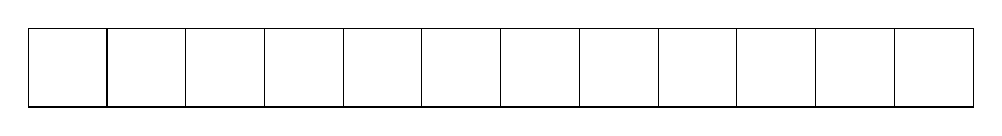
\begin{tikzpicture}
        \foreach \x in {1,...,12} {
            \draw (\x,0) rectangle (\x+1,1);
            \node at (\x+0.5,0.5) {};
        }
    \end{tikzpicture}
\end{center}
So to insert a key $k$, we consider a sequence of random hashes $h_1(k), h_2(k), \ldots$ and each $h_i(k)$ is uniformly random in $1, \ldots, n$ and $h_i$'s are independent. We place the key in the first available position out of the sequence $h_1, h_2, h_3, \ldots$. 

\noindent To query $k$, we try $h_1(k), h_2(k), \ldots$ until 
\begin{itemize}
    \item we find $k$, in which case we return true.
    \item or we find a free slot, in which case we return false.
\end{itemize}
Observations:
\begin{enumerate}
    \item If the hash table is $1 - \delta$ full, then 
    \begin{align*}
        E[\text{time for next insertion}] = \delta^{-1}.
    \end{align*}
    \item Suppose I fill $1-\epsilon$ full. Then,
    \begin{align*}
        E[\text{time to query random elements of those present}] &\approx \frac n2 \cdot O(2) + \frac n4 \cdot O(4) + \frac n8 \cdot O(8) + \cdots + \epsilon n \cdot O(\epsilon^{-1})\\
        &\approx \underbrace{1 + 1 + \cdots + 1}_{\lg \epsilon^{-1} \text{ terms}} \\
        &= O(\lg \epsilon^{-1}).
    \end{align*}
\end{enumerate}
``Open-addressed hash tables'': Any hash table that is ``like random-probing'' but that possibly uses a different distribution for its probe sequence
\begin{align*}
    h_1(k), h_2(k), \ldots
\end{align*}
Some examples include linear probing and double hashing. 

\newpage
% create conjecture env
\clm{Ullman '72}{
    For any open address hash table, 
    \begin{align*}
        E[\text{time to query rnadom elements of those present}] \geq \Omega(\lg \epsilon^{-1}).
    \end{align*}
}
\noindent This was proven by Andrew Yao in 1985. The title of his paper was ``Uniform Hashing is Optimal.'' He ended the paper with the following conjecture:
\clm{Yao '85}{
    For any open address hash table, if you fill it to $(1-\epsilon)$ full, the expected time of the next insertion is at least $\Omega(\epsilon^{-1})$. 
}
\thm{}{
    Possible to achieve 
    \begin{align*}
        E[\text{insertion time}] = O( \lg^2 \eps^{-1}).
    \end{align*}
}
\noindent We now turn attention towards the coupon collector problem:
\qs{Coupon Collector}{We have a hat with $n$ coupons in it. We repeatedly draw random coupons from it, with replacement. The classical question is how many draws in expectation do we need to collect all $n$ coupons? The answer to this is $O(n \log n)$.}
\thm{}{Let $\delta \in (0, 1)$ be such taht $\delta \geq \frac{1}{n^{1/10}}$. Let $X$ be the number of draws until we have collected a $(1-\delta)$ fraction of all the coupons. Then, with high probability, $X \leq 2n\ln \delta^{-1}$. }
\begin{proof}
    Do $2n \ln \delta^{-1}$ draws. Let $Y$ be the number of distinct coupons not sampled. Then,
    \begin{align*}
        E[Y] &= \sum_{i=1}^n P(\text{coupon $i$ is not sampled}) \\
        &=  n \cdot \left(1  - \frac 1n\right)^{2n \ln \delta^{-1}} \\
        &\approx n \delta^2.
    \end{align*}
    Applying McDiarmid's to $Y$,
    \begin{itemize}
        \item $Y$ is a function of $m = 2n \ln \delta^{-1}$ random variables.
        \item Each of these random variables can only affect $Y$ by $\pm 1$. 
    \end{itemize}
    So by McDiarmid's, we have with high probability that
    \begin{align*}
        &Y \leq E[Y] + \tilde{O}(\sqrt m) \\
        &\implies Y \leq \delta^2 n + \tilde{O}(\sqrt m) \\
        &\implies \text{number of sampled coupons} \geq n - \underbrace{(\delta^2 n + \tilde O(\sqrt m))}_{\lll \delta n} \\
        & \geq (1-\delta)n.
    \end{align*}
\end{proof}
\newpage
\noindent We now learn about a new hash table design. Break up the table as follows:
\begin{itemize}
    \item $p_1$ is the first $\frac n2$ slots.
    \item $p_2$ is the next $\frac n4$ slots.
    \item $\vdots$
    \item Do this until there is a $\epsilon n / 100$ size part.
\end{itemize}
Probe sequence:
\begin{itemize}
    \item Try $100 \lg \epsilon^{-1}$ probes in $p_1$.
    \item Try $100 \lg \eps^{-1}$ probes in $p_2$.
    \item $\vdots$
\end{itemize}
If this fails for all parts, 
\begin{itemize}
    \item Do $100 \log n$ probes in the final part.
    \item Loop through the array until there is a free spot in the worst case.
\end{itemize}
The most recent step happens with very very low probability, but is required for correctness of the data structure. 

Now suppose $p_i$ gets $\geq 50\%$ full for some $i$. This means that $p_{i-1}$ must have gotten at least $\frac{|p_i|}{2} \cdot 100 \lg \epsilon^{-1}$ probes. So, with high probability, if $p_i$ gets $50\%$ full, we have that 
\begin{align*}
    \frac{|p_i|}{2} \cdot 100 \lg \epsilon^{-1} = |p_{i-1}| \cdot 25 \lg \epsilon^{-1},
\end{align*}
which means that $p_{i-1}$ is $1 - \epsilon^{12.5}$ full. Then $p_{i-2}$ is also at least $1 - \eps^{12.5}$ full, and all $p_{i-1}, p_{i-2}, \ldots, p_1$ are all at least $1-\eps^{12.5}$ full. We claim that the final part is $\leq \frac 12$ full. This is because if the final part were $\geq \frac 12$ full, then all the earlier parts would be $\geq 1-\eps^{12.5}$ full, meaning that the overall number of elements is 
\begin{align*}
    &\geq  (1 - \eps/10) (|p_1| + \cdots + |p_{k}|) \\
    &= n \cdot \left( 1 - \frac \eps {50}\right) \\
    &> (1-\eps)n.
\end{align*}
But this yields a contradiction, meaning the final part never reaches $50\%$ full. As such, we have disproved Yao's claim. So,
\begin{itemize}
    \item Once we get to the final part, the expected additional time is $O(1)$. 
    \item So, the total expected time is 
    \begin{align*}
        O(1) + \text{number of probes before final part} \\
        = O(1) + 100 \lg \eps^{-1} \cdot O(\lg \eps^{-1}) = O(\lg^2 \eps^{-1}).
    \end{align*}
\end{itemize}
\newpage
\section{Linear Probing}
To insert an element $v$ into a hash table that incorporates linear probing, we just
\begin{itemize}
    \item place $v$ in the first free slot out of $h(v), h(v) + 1, \ldots$ (modulo the table size).
\end{itemize}
Searching for an element $v$ uses the same process. At relatively low capacity, linear probing is the most efficient hash table known to man.
But now suppose we perform $(1 - 1/x)\cdot n$ insertions and perform one more insertion.
\clm{Peterson 1957}{
    The expected insertion time is $O(x)$. 
}
\thm{Knuth 1962}{
    The expected insertion time is $\Theta(x^2)$.
}
\noindent Intuition for clustering:
\begin{itemize}
    \item The longer your run gets, the more likely you are to hash into the run. ``Winner keeps winning.''
    \item ``Globbing effect.'' This is when an insertion connects two clusters. 
\end{itemize}
\noindent Intuition \#2:
\begin{itemize}
    \item Consider an interval $I$ with size $x^2$. Let $R$ be the number of items whose hashes are in $I$. We consider properties of $R$. So first,
    \begin{align*}
        E[R] &= (1-1/x)\cdot x^2 = x^2 - x \\
        \mathrm{std} (R) &\approx \sqrt{E[R]} \approx x.
    \end{align*}
    Moral: intervals of size $\leq x$ often have more elements hashing to them than can fit. 
\end{itemize}
\mlenma{}{
    Throw $(1-1/x)\cdot n$ balls into $n$ bins. Let $k > 0$. Define $P_i$ to be the number of balls in the first $i$ bins. Then
    \begin{align*}
        P(\exists \text{ any $i \geq kx^2$ such that } P_i \geq i) \leq e^{-\Omega(k)}.
    \end{align*}
    Call the event above $*$.
}
\noindent Warmup: What is $P(P_{kx^2} \geq kx^2)$? (call this event $\dagger$)
\begin{align*}
    \mu = E[P_{kx^2}] = (1-1/x) \cdot kx^2  = kx^2 - kx.
\end{align*}
So $\sqrt \mu \leq \sqrt{kx^2} = \sqrt k x$.So,
\begin{align*}
    P(P_{kx^2} \geq kx^2) \approx P(P_{kx^2} \geq \mu + \sqrt k \sqrt \mu) = e^{-\Omega(k)}.
\end{align*}
Now we make a critical claim. If we condition on any prefix being problematic, then
\begin{align*}
    P(\dagger \mid *) = \Omega(1).
\end{align*}
This would mean that $P(*) = \Theta(P(\dagger))$, so by the warmup, we'd be done.
\begin{proof}
    Assume event $*$. Let $i$ be the largest $i$ such that $P_i \geq i$. Note that $kx^2 \leq i$ because we assumed $*$. If you tell me $I, P_i$, what is the conditional distribution for $P_{kx^2}$. Then,
    \begin{align*}
        P_{kx^2} \sim \text{binomial random variable given by sum of $P_i$ balls,} \\
        \text{ each of which has probability $kx^2/i$ of landing in the first $kx^2$ bins.}
    \end{align*}
    Therefore, $P_{kx}$ is now a binomial random variable with mean $P_i \cdot \frac{kx^2}{i} \geq kx^2$. Any binomial random variable with mean $\mu \geq 1$ has $\Omega(1)$ probability of meeting or exceeding its mean. So it follows that $P(\dagger \mid *) \geq \Omega(1)$.  This completes the proof of the lemma.
    \newpage
    \noindent Returning to Knuth's theorem, consider insertion of an element $u$ at $(1 - 1/x)$ full. Then we want to show that
    \begin{align*}
        P(\text{insertion time} \geq kx^2) \leq e^{-\Omega(k)}.
    \end{align*}
    Now consider a table where the range $[h(v) -r, h(v) + kx^2)$ is saturated. Then, there exists a suffix of array slots ending at slot $h(v) + kx^2 - 1$ such that 
    \begin{itemize}
        \item $|\text{suffix}| \geq kx^2$
        \item the number of elements that hash to suffix $\geq |\text{suffix}|$.
    \end{itemize}
    This is where we apply the lemma. This directly gives us that 
    \begin{align*}
        P(\text{insertion time} \geq kx^2) \leq e^{-\Omega(k)}
    \end{align*}
    which completes the proof.  
\end{proof}

\section{Ordered Linear Probing}

\thm{Knuth 1963}{Suppose you fill a linear-probing hash table to $(1 - 1/x)$ full. Then, the expected insertion time is $\Theta(x^2)$.}
\noindent Amble and Knuth had the following idea:
modify the hash table such that in each ``run'', maintain an invariant that the elements in the run are in sorted order by hash.

\noindent Aside: if elements have the same hash, imagine we break ties with another hash function. 
\nt{
    Also note that this is a history-independent data structure, meaning that the final state of the hash table is independent of the order of the elements added. 
}
\thm{Amble and Knuth 1973}{
    $E[\text{time to query an element}] = O(x)$. 
}
\begin{proof}
    Just to simplify things, we will assume positive queries, meaning we only query elements that exist in the hash table.  

    Let $S = \{\text{elements in the hash table}\}$. For $s \in S, Q_s$ is the query time for $s$. Also define $I_s$ as the insertion time for $s$ when it was inserted.

    \noindent \textbf{Observation 1}: $E[Q_s]$ is the same $\forall s\in S$.
    
    \noindent \textbf{Proof}: By symmetry and because the hash table is history-independent. $\hfill \qed$

    \noindent \textbf{Observation 2}: 
    \begin{align*}
        \sum_{s\in S} Q_s = \sum_{s \in S} I_s.
    \end{align*}
    \noindent \textbf{Proof}: Just think about it lowkey. Basically if the insertion time is $k$, then we increase the sum of the query times by $k$.  $\hfill \qed$

    \noindent \textbf{Observation 3}: 
    \begin{align*}
        E\left[ \sum_{s \in S} I_s \right] = \Theta(n \cdot x).
    \end{align*}
    \noindent \textbf{Proof}: Well we have 
    \begin{align*}
        E\left[ \sum_{s \in S} I_s \right] &= \Theta \left( \frac n2 \cdot 2^2 + \frac n4 \cdot 4^2 + \frac n8 \cdot 8^2 + \cdots + \frac{n}{x} \cdot x^2\right) \\
        &= \Theta\left( n\cdot x\right). \tag{dominated by last summand}
    \end{align*}
    This completes the proof of the observation. $\hfill \qed$

    \noindent Moving to the proof of the theorem, we have:
    \begin{align*}
        E[Q_s] &= \frac{1}{|S|} \cdot \sum_{s \in S} E[Q_s] \\
        &= \frac{1}{|S|} \cdot \sum_{s \in S} E[I_s] \\
        &= \frac{1}{\Theta(n)} \cdot \Theta(n \cdot x) \\
        &= \Theta(x).
    \end{align*}
\end{proof}
\subsection{Deletions}
Idea: use ``tombstones.'' That is, rather than entirely deleting the element, we just mark the index as ``deleted.'' What that means is that when we query that index, all we know is that there used to be an element at that spot. Also when trying to insert an element, the tombstone spot is just as good as any other open spot to insert the element. 

However, queries cannot treat tombstones are empty. This is because the element we are searching for could still be to the right of a tombstone. So queries skip over tombstones. 

Every so often, we should pause and rebuild the hash table, but with the tombstones removed. How often? The classical measure is every $R =  \frac{n}{2x}$ operations. 

\noindent \textbf{Question}: What if we have a table with insertions and deletions?

\noindent Experiment: initially fill our hash table to $1 - 1/x$ full. Then, we alternate between insertions and deletions. We get this graph:

\begin{center}
    \includegraphics*[width=15cm]{hashtableexperiment.jpg}
\end{center}
\newpage
\thm{Kuszmaul (2022)}{
    Consider any workload such that the hash table is never $> 1-1/x$ full. Then, the amortized expected time per operation is $\widetilde O(x)$. The actual optimal bound is $\Theta(x \lg^{1.5} x)$. 
}
\noindent \textbf{Big Idea 1}: Consider all the opeartions in a given rebuild window. Then we draw a random line in the hash table and ask how many insertions crossed the line. If we can answer this for every dotted line, we can sum to get the sum of the insertion times. 

\noindent \textbf{Big Idea 2}: Before rebuilding, consider the state of the hash table.
Draw an X in every empty slot before the random line. Then for every deletion that occurs in the rebuild window, we draw an X at the time of deletion and at the position of the deleted element. Similarly for insertions, but use $\checkmark$. Now we draw a path from the bottom left to the top right of the graph (nondecreasing). It turns out that 
\begin{align*}
    \text{the number of insertions that cross the line} = \max_{\text{all possible paths }p} (\text{number of $\checkmark$ under path } - \text{ number of X under path}).
\end{align*}
\noindent \textbf{Big Idea 3}: With enough work, we get a simpler problem which we call the \underline{path surplus problem}. That is, we have an $x \times x$ grid where each entry is randomly $\pm 1$. Consider every monotonic path to the right. For each path $p$, we have 
\begin{align*}
    \mathrm{surplus}(p) = \sum \text{ entries under $p$}.
\end{align*}
The question is what is the expected max surplus over all path? 
\thm{}{
    The expected maximum surplus is $\Theta(x \lg^{0.75} x)$. 
}

\end{document}